\documentclass[twocolumn,10pt]{article}
\usepackage[letterpaper,left=1.95cm,right=1.95cm,top=2.5cm,bottom=3.16cm]{geometry}
\usepackage{natbib}
\usepackage{hyperref}
\usepackage{float}
\usepackage{graphicx}
\usepackage{ragged2e}
\usepackage{booktabs}
\usepackage{amsmath}
\input{parametros.sty}
\raggedbottom % evita que LaTeX estire el espacio vertical para llenar columnas (huecos en blanco)

\setcitestyle{numbers,square}
\graphicspath{{Figuras/}}
\lhead{HealthTech 1 y 2}
\rhead{Proyecto Final HealthTech, p\'agina \thepage\ de \pageref{LastPage}}
\newcommand{\ra}{\textsuperscript{a}}

%%%%%%% ENCABEZADO %%%%%%%%%%%%%%%%%%%%
\title{\fontsize{15}{17}\selectfont
\vspace*{-0.7cm}
\textbf{Factores de riesgo cardiovascular y predicci\'on de enfermedad coronaria: un enfoque de ciencia de datos con regresi\'on log\'istica y \'arboles de decisi\'on en pacientes remitidos a angiograf\'ia}\\[0.25cm]
\fontsize{11}{13}\selectfont
\textbf{Cardiovascular risk factors and prediction of coronary artery disease: a data science approach using logistic regression and decision trees in patients referred for angiography}\\[0.2cm]}

\author{
  \begin{tabular}{c}
    \textbf{Angie Milena Tobar Aguirre}\\
    \small Pregrado en Ciencia de Datos, Universidad Externado de Colombia\\
    \small \texttt{angie.tobar@est.uexternado.edu.co}
  \end{tabular}
  \and
  \begin{tabular}{c}
    \textbf{Alejandro Pardo Costo}\\
    \small Pregrado en Ciencia de Datos, Universidad Externado de Colombia\\
    \small \texttt{alejandro.pardo2@est.uexternado.edu.co}
  \end{tabular}
}
\date{}

\begin{document}

\twocolumn
[
\begin{@twocolumnfalse}
\maketitle
\begin{abstract}
\vspace*{0.3cm}
\justify
\fontsize{9.5pt}{11pt}\selectfont
\textbf{Antecedentes.} La enfermedad coronaria (EC) es la principal causa de muerte en el mundo y su confirmaci\'on requiere angiograf\'ia, un procedimiento invasivo y costoso. \textbf{Objetivo.} Caracterizar los factores de riesgo cardiovascular y los hallazgos cl\'inicos asociados a la EC angiogr\'afica y evaluar la discriminaci\'on y calibraci\'on de modelos de regresi\'on log\'istica y \'arboles de decisi\'on. \textbf{M\'etodos.} Estudio observacional anal\'itico de corte transversal con la base oficial UCI \textit{Heart Disease} (Cleveland; 303 pacientes; 297 con datos completos y 137 eventos). Se auditaron los datos, se estimaron OR por rangos cl\'inicos y OR ajustados por regresi\'on log\'istica con verificaci\'on de supuestos, y se compararon una regresi\'on log\'istica b\'asica (11 variables no invasivas), una extendida (con fluoroscopia y gammagraf\'ia con talio), un \'arbol CART y un Random Forest mediante validaci\'on cruzada estratificada $5\times20$, bootstrap de optimismo, AUC con IC de DeLong y calibraci\'on. \textbf{Resultados.} Fueron predictores independientes el dolor tor\'acico asintom\'atico (OR 10,60; IC 95\,\% 3,17--35,40), el sexo masculino (OR 7,48; 3,25--17,20) y la depresi\'on del ST (OR 1,82 por mm; 1,23--2,69); la frecuencia card\'iaca m\'axima fue protectora con significancia lim\'itrofe (OR 0,82 por 10\,lpm; $p=0{,}048$). El colesterol no se asoci\'o de forma independiente. El modelo b\'asico alcanz\'o un AUC de 0,874 (0,880 corregido por optimismo) con pendiente de calibraci\'on de 0,91; la imagen aport\'o un $\Delta$AUC de 0,035 ($p=0{,}012$). La regresi\'on log\'istica super\'o al \'arbol ($\Delta$AUC 0,067; $p=0{,}004$) e igual\'o al Random Forest. La versi\'on de Kaggle de la base, usada en una fase previa, ten\'ia la etiqueta diagn\'ostica invertida. \textbf{Conclusi\'on.} Las variables cl\'inicas de bajo costo discriminan bien la EC angiogr\'afica; un modelo log\'istico simple y bien calibrado es preferible a algoritmos m\'as complejos en esta poblaci\'on.

\keywordsSpan{enfermedad coronaria; factores de riesgo cardiovascular; regresi\'on log\'istica; \'arboles de decisi\'on; validaci\'on cruzada; calibraci\'on.}
\end{abstract}

\renewcommand{\abstractname}{ABSTRACT}
\begin{abstract}
\vspace*{0.2cm}
\justify
\fontsize{9.5pt}{11pt}\selectfont
Coronary artery disease (CAD) is the leading cause of death worldwide and its confirmation requires invasive angiography. Using the official UCI \textit{Heart Disease} Cleveland dataset (297 complete cases, 137 events), we estimated crude and adjusted odds ratios and compared a basic logistic regression (11 non-invasive variables), an extended model (adding fluoroscopy and thallium scintigraphy), a CART tree and a Random Forest through repeated stratified $5\times20$ cross-validation, optimism bootstrap, DeLong confidence intervals and calibration. Asymptomatic chest pain (OR 10.60), male sex (OR 7.48) and exercise ST depression (OR 1.82 per mm) were independent predictors. The basic model reached an AUC of 0.874 (0.880 optimism-corrected) with good calibration; imaging added 0.035. Logistic regression outperformed the tree and matched the Random Forest. The widely used Kaggle version of the dataset has an inverted diagnostic label.

\keywordsEng{coronary artery disease; cardiovascular risk factors; logistic regression; decision trees; cross-validation; calibration.}
\end{abstract}
\vspace*{0.4cm}
\end{@twocolumnfalse}
]

%======================================================================
\section{Introducci\'on}
%======================================================================
\justifying
Las enfermedades cardiovasculares causaron 19,2 millones de muertes en 2023, una de cada tres en el mundo \cite{ihme2025}. Se estiman unos 315 millones de casos prevalentes de EC \cite{stark2024}, y en Colombia las cuatro enfermedades cardiovasculares m\'as frecuentes afectan a 5,6 millones de personas \cite{deloitte2015}. Un evento coronario cuesta entre \$17 y \$29 millones COP seg\'un la comorbilidad, y el costo cae m\'as del 80\,\% despu\'es de la fase aguda \cite{rcc2018}.

La EC es el estrechamiento de las arterias coronarias por placa ateroscler\'otica. Su diagn\'ostico es escalonado: historia cl\'inica, electrocardiograma (ECG), prueba de esfuerzo, imagen funcional y, finalmente, angiograf\'ia coronaria, que es el est\'andar de referencia \cite{vrints2024}. Desde Diamond y Forrester se sabe que la edad, el sexo y el tipo de dolor tor\'acico permiten estimar la probabilidad pretest de la enfermedad \cite{diamond1979}. Detrano \textit{et al.} desarrollaron con los datos de Cleveland un algoritmo de probabilidad aplicado en cuatro centros \cite{detrano1989}, y el CAD Consortium mostr\'o que las reglas cl\'asicas sobrestiman la prevalencia actual \cite{genders2011}.

La base de Cleveland es una de las m\'as usadas para ense\~nar clasificaci\'on, con exactitudes reportadas superiores al 90\,\% sobre particiones de unos 60 pacientes \cite{chandrasekhar2023}. Sin embargo, persisten tres problemas: (i) evaluaciones con una sola partici\'on peque\~na, muy inestables; (ii) omisi\'on de la calibraci\'on, que es indispensable para un uso cl\'inico \cite{vancalster2019}; y (iii) mezcla de variables de consulta con variables de imagen, que impide saber cu\'anto discriminan por s\'i solas las variables de bajo costo. \textbf{Este estudio cubre ese vac\'io}: cuantifica el desempe\~no de las variables no invasivas y el valor incremental de la imagen con validaci\'on interna rigurosa, siguiendo TRIPOD \cite{collins2015}.

\textbf{Pregunta de investigaci\'on.} En adultos remitidos a angiograf\'ia por sospecha cl\'inica, ?`qu\'e factores de riesgo y hallazgos no invasivos se asocian de forma independiente con la EC angiogr\'afica, y con qu\'e discriminaci\'on y calibraci\'on la predicen modelos de regresi\'on log\'istica y \'arboles de decisi\'on, con y sin variables de imagen?

\subsection{Problema y justificaci\'on}
En la cohorte, 160 de 297 pacientes remitidos a angiograf\'ia (53,9\,\%) no ten\'ian EC.
\begin{itemize}
\item \textbf{Causas:} s\'intomas at\'ipicos o silentes (el 47,8\,\% era asintom\'atico), informaci\'on cl\'inica dispersa y estimaci\'on subjetiva del riesgo.
\item \textbf{Consecuencias:} procedimientos invasivos innecesarios, diagn\'osticos tard\'ios y uso ineficiente de la hemodinamia.
\item \textbf{Alternativa:} integrar en un modelo validado las variables disponibles antes de la angiograf\'ia.
\item \textbf{Beneficiarios:} pacientes y m\'edicos (directos); IPS, EPS y sistema de salud (indirectos).
\end{itemize}

\subsection{Objetivos}
\textbf{General.} Caracterizar los factores de riesgo cardiovascular y los hallazgos cl\'inicos asociados a la EC angiogr\'afica en 297 pacientes remitidos a angiograf\'ia, y evaluar el desempe\~no predictivo (discriminaci\'on y calibraci\'on) de modelos de regresi\'on log\'istica y \'arboles de decisi\'on.

\textbf{Espec\'ificos.}
\begin{enumerate}
\item[OE1.] Describir las caracter\'isticas de la cohorte seg\'un la presencia de EC.
\item[OE2.] Determinar la asociaci\'on cruda (OR por rangos) y ajustada (regresi\'on log\'istica) de cada factor con la EC.
\item[OE3.] Desarrollar y validar internamente modelos de regresi\'on log\'istica, \'arbol de decisi\'on y Random Forest, y evaluar su desempe\~no.
\item[OE4.] Cuantificar el valor incremental de la fluoroscopia y de la gammagraf\'ia con talio.
\item[OE5.] Contrastar los resultados con la literatura.
\end{enumerate}

\subsection{Hip\'otesis}
\textbf{General:} los factores de riesgo y los hallazgos de consulta, ECG y prueba de esfuerzo predicen la EC con un desempe\~no cl\'inicamente aceptable. Se contrastan cuatro pares de hip\'otesis ($\alpha=0{,}05$):
\begin{itemize}
\item \textbf{H-1} (OE2). H0: todos los $\beta_j=0$ en el modelo b\'asico. H1: al menos un $\beta_j\neq0$.
\item \textbf{H-2} (OE3). H0: AUC$_{\text{b\'asico}}\leq0{,}80$. H1: AUC$_{\text{b\'asico}}>0{,}80$.
\item \textbf{H-3} (OE4). H0: AUC$_{\text{ext}}=$ AUC$_{\text{b\'asico}}$. H1: AUC$_{\text{ext}}>$ AUC$_{\text{b\'asico}}$.
\item \textbf{H-4} (OE3). H0: AUC$_{\text{CART}}=$ AUC$_{\text{RL ext}}$. H1: los AUC difieren.
\end{itemize}

%======================================================================
\section{Metodolog\'ia}
%======================================================================
\subsection{Dise\~no, poblaci\'on y muestra}
\begin{itemize}
\item \textbf{Dise\~no:} estudio aplicado, cuantitativo, observacional anal\'itico de corte transversal, con datos secundarios y desarrollo y validaci\'on interna de un modelo diagn\'ostico (TRIPOD tipo 1b \cite{collins2015}).
\item \textbf{Universo:} adultos con sospecha de EC.
\item \textbf{Poblaci\'on:} pacientes remitidos a angiograf\'ia en la Cleveland Clinic Foundation (Ohio, EE.\,UU.), con datos donados a UCI en 1988 \cite{detrano1989,uci1988}.
\item \textbf{Unidad de an\'alisis:} el paciente.
\item \textbf{Muestreo:} censo de los 303 registros, que corresponden a pacientes consecutivos (no probabil\'istico).
\item \textbf{Inclusi\'on:} angiograf\'ia y 13 predictores completos. \textbf{Exclusi\'on:} faltantes en \texttt{ca} ($n=4$) o en \texttt{thal} ($n=2$). Muestra anal\'itica: $n=297$ (Fig.~\ref{fig:flujo}).
\item \textbf{Desenlace:} EC angiogr\'afica, es decir, estenosis $>50$\,\% en al menos un vaso mayor (\texttt{num}~$\geq1$).
\end{itemize}

\begin{figure}[H]
\centering
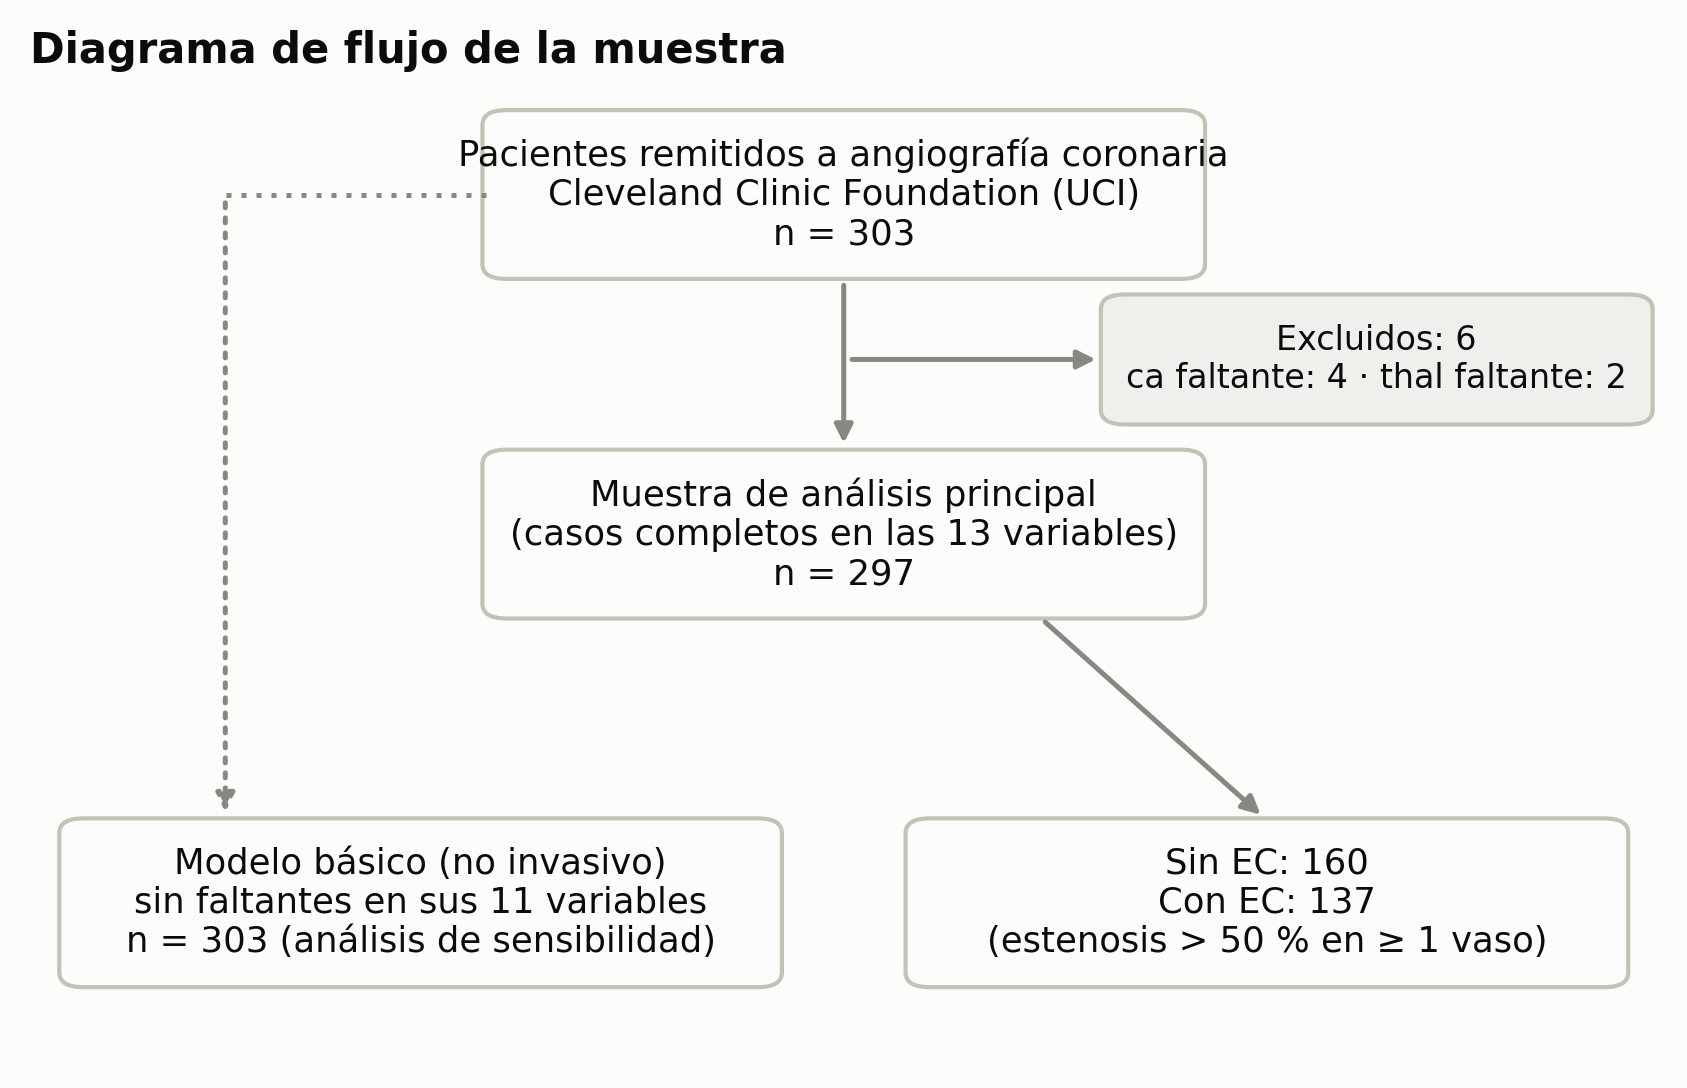
\includegraphics[width=\columnwidth]{fig02_flujo_muestra.png}
\caption{Diagrama de flujo de la muestra. La l\'inea punteada indica el an\'alisis de sensibilidad con $n=303$.}
\label{fig:flujo}
\end{figure}

\textbf{Tama\~no de muestra.} Seg\'un los criterios de Riley \textit{et al.} \cite{riley2020} (contracci\'on $\geq0{,}90$; optimismo del $R^2$ $\leq0{,}05$; prevalencia $\pm0{,}05$), se requer\'ian $n=412$ para el modelo b\'asico (14 par\'ametros) y $n=382$ para el extendido (17). Con $n=297$ hay 9,8 y 8,1 eventos por par\'ametro. Se declara como limitaci\'on y se mitiga con penalizaci\'on L2, validaci\'on cruzada repetida, correcci\'on de optimismo y reporte de la pendiente de calibraci\'on.

\subsection{Variables}
\begin{itemize}
\item \textbf{Factores de riesgo:} edad, sexo, presi\'on arterial sist\'olica en reposo (PAS), colesterol total y glucemia en ayunas $>120$\,mg/dL.
\item \textbf{Marcadores cl\'inicos:} tipo de dolor tor\'acico, ECG de reposo (colapsado a normal/anormal porque la anomal\'ia ST-T tiene $n=4$), frecuencia card\'iaca (FC) m\'axima, angina de esfuerzo, depresi\'on del ST y pendiente del ST.
\item \textbf{Imagen:} vasos coloreados por fluoroscopia (\texttt{ca}) y gammagraf\'ia con talio (\texttt{thal}).
\end{itemize}
La definici\'on conceptual y operacional de cada variable est\'a en el anexo del repositorio (\texttt{docs/diccionario\_variables.md}).

\subsection{Control de calidad de los datos}
Se us\'o el archivo oficial \texttt{processed.cleveland.data}, verificado por SHA-256, y se aplicaron controles de rango fisiol\'ogico, de c\'odigos v\'alidos y de duplicados: no se encontr\'o ning\'un valor fuera de rango, ning\'un c\'odigo inv\'alido ni ning\'un duplicado. Adem\'as se audit\'o la versi\'on de Kaggle usada en la fase previa del proyecto, emparejando registro a registro:
\begin{itemize}
\item la etiqueta \texttt{target} est\'a \textbf{invertida en el 100\,\% de los casos};
\item \texttt{cp}, \texttt{restecg} y \texttt{slope} est\'an recodificadas;
\item hay faltantes ocultos como \texttt{ca}~$=4$ y \texttt{thal}~$=0$;
\item hay un registro duplicado (Fig.~\ref{fig:auditoria}).
\end{itemize}

\begin{figure}[H]
\centering
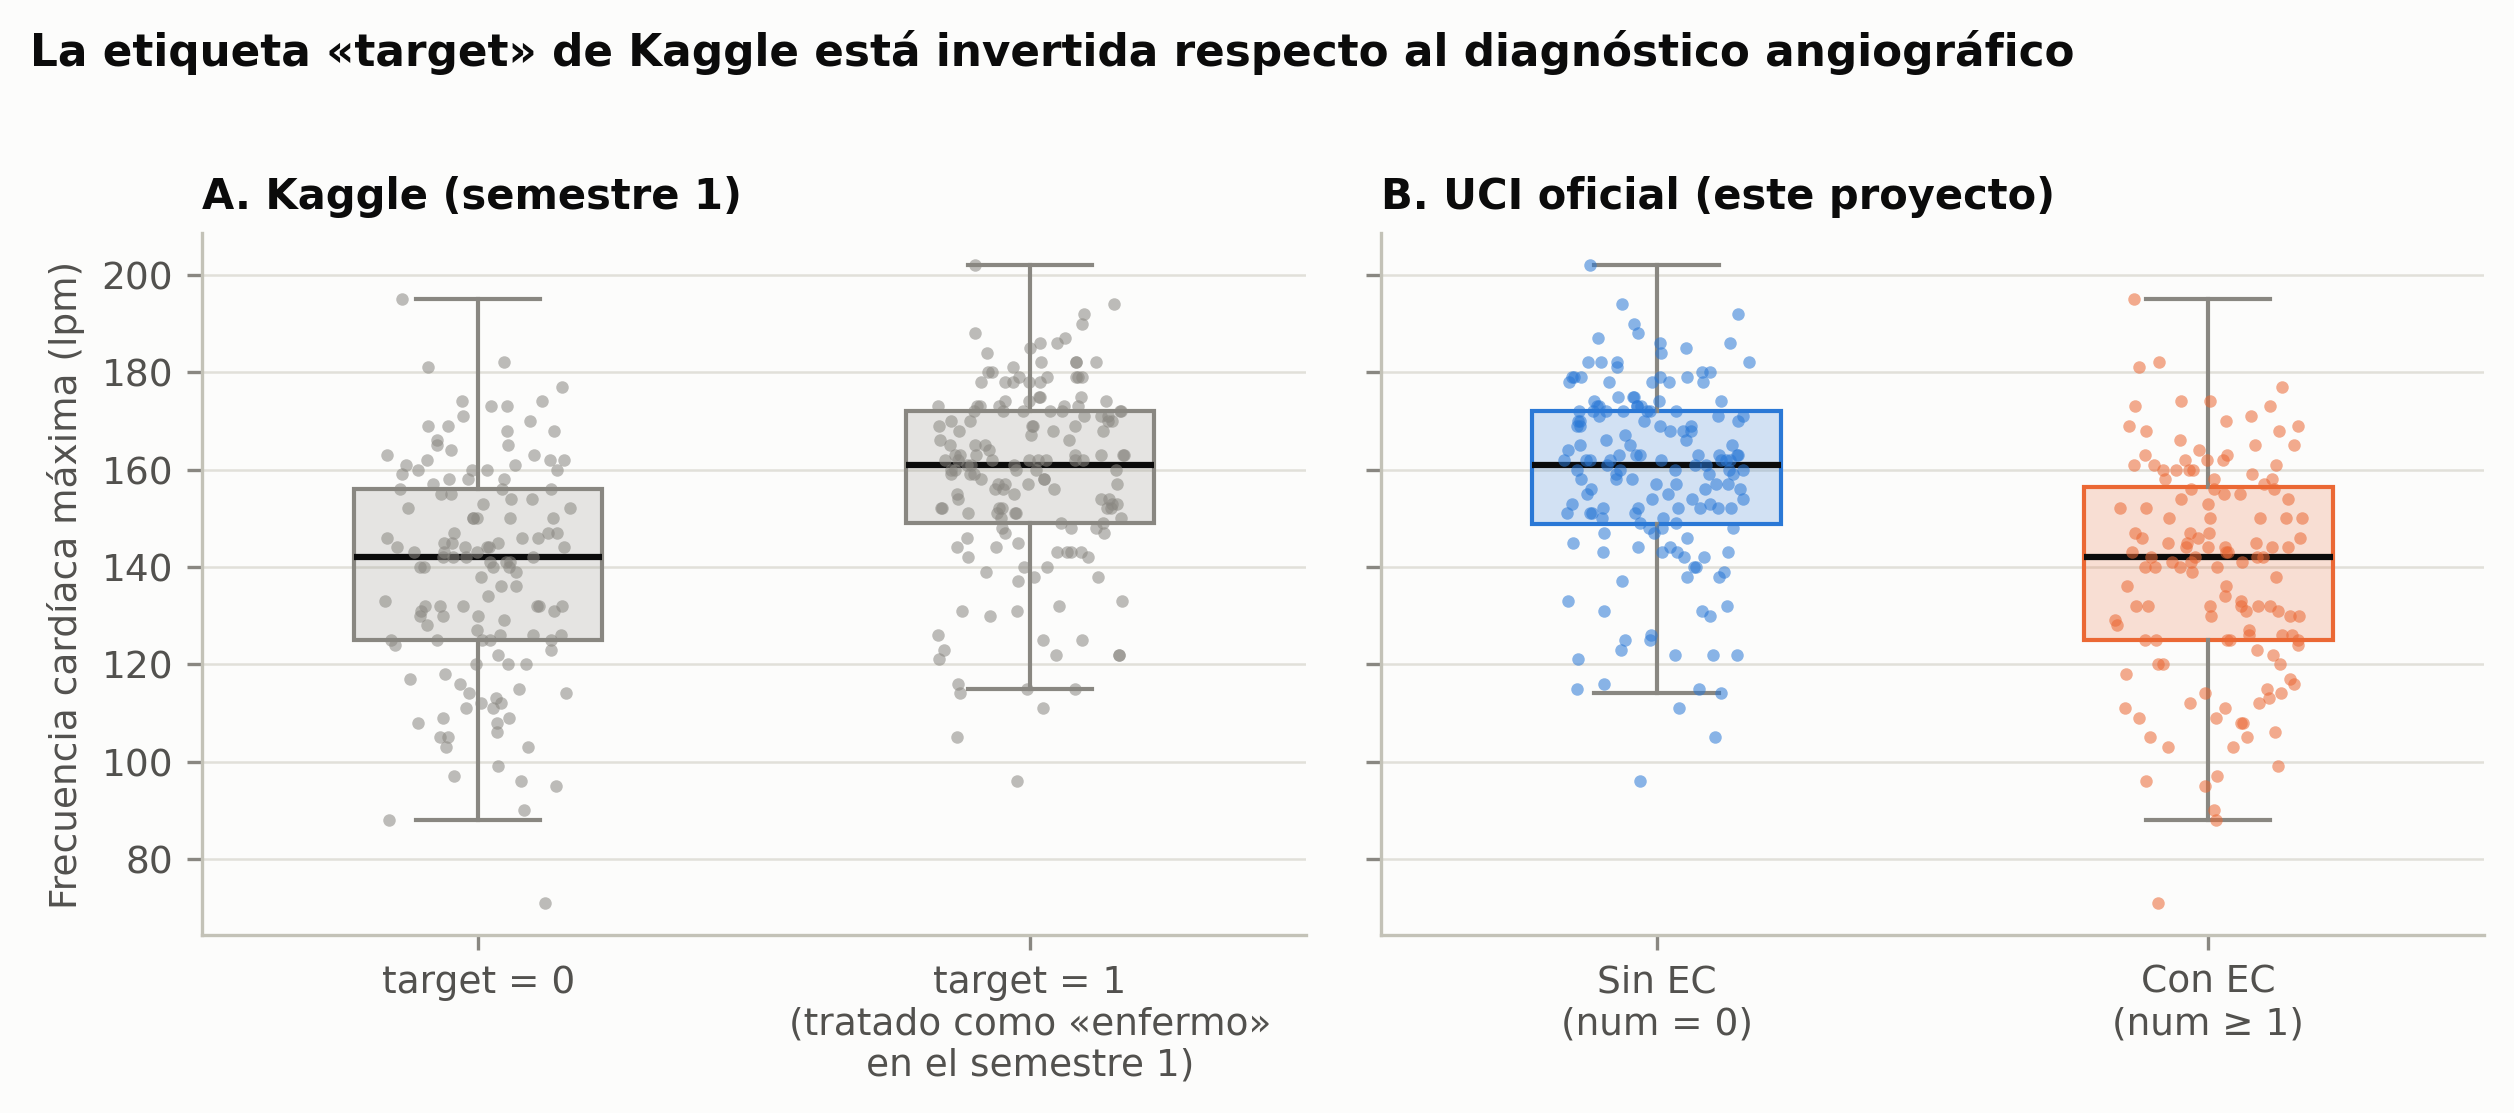
\includegraphics[width=\columnwidth]{fig01_auditoria_kaggle_vs_uci.png}
\caption{FC m\'axima seg\'un la etiqueta de Kaggle (A) y la oficial (B). Con la etiqueta oficial, los pacientes con EC alcanzan menor FC, como se espera fisiol\'ogicamente.}
\label{fig:auditoria}
\end{figure}

\subsection{An\'alisis estad\'istico}
\textbf{Descriptivo.} Se evalu\'o la normalidad con Shapiro-Wilk \cite{shapiro1965} en cada grupo. Las continuas se compararon con U de Mann-Whitney (correlaci\'on biserial por rangos) o t de Welch, y las cualitativas con $\chi^2$ de Pearson (V de Cram\'er), exacta de Fisher o $\chi^2$ por Monte Carlo cuando alg\'un esperado era $<5$.

\textbf{Paso preliminar.} Seg\'un el tipo de variable dependiente (Y continua: regresi\'on lineal; Y binaria: log\'istica), se ajustaron dos modelos de m\'inimos cuadrados: un modelo lineal de probabilidad (MLP) sobre la EC y una regresi\'on de la PAS sobre la edad, el sexo, el colesterol y la glucemia. Sus supuestos se verificaron con Shapiro-Wilk sobre los residuos y con Breusch-Pagan.

\textbf{Asociaci\'on.}
\begin{itemize}
\item \textbf{OR por rangos} con cortes cl\'inicos fijados de antemano: OR~$=ad/bc$, con IC de Woolf.
\item \textbf{Regresi\'on log\'istica} por m\'axima verosimilitud sin penalizar: OR crudos y ajustados (modelos b\'asico y extendido), con IC de Wald.
\item \textbf{Supuestos:} linealidad del logit (Box-Tidwell), colinealidad (VIF), bondad de ajuste (Hosmer-Lemeshow \cite{hosmer2013}) e influencia (distancia de Cook).
\end{itemize}

\textbf{Modelos predictivos} (scikit-learn \cite{pedregosa2011}):
\begin{enumerate}
\item[M0.] Regresi\'on log\'istica (RL) con 4 variables continuas, como l\'inea base de la fase previa.
\item[M1.] RL b\'asica (11 variables no invasivas).
\item[M2.] RL extendida (13 variables). En M0--M2: penalizaci\'on L2, $C=1$, variables estandarizadas.
\item[M3.] \'Arbol CART con criterio de Gini \cite{breiman1984}; profundidad $\in\{2,\dots,5\}$ y tama\~no m\'inimo de hoja $\in\{5,10,20\}$, elegidos por validaci\'on cruzada anidada.
\item[M4.] Random Forest \cite{breiman2001} con 300 \'arboles y hojas de al menos 5 pacientes.
\end{enumerate}

\textbf{Validaci\'on.}
\begin{itemize}
\item Validaci\'on cruzada estratificada repetida $5\times20$, con las mismas 100 particiones para todos los modelos.
\item Bootstrap de optimismo de Harrell con 500 r\'eplicas \cite{harrell2015}.
\item AUC con IC de DeLong \cite{delong1988,sun2014}.
\item Calibraci\'on: pendiente, intercepto y Brier \cite{vancalster2019}.
\item Sensibilidad, especificidad, VPP y VPN con umbral 0,5 y con el umbral que garantiza una sensibilidad $\geq90$\,\%.
\item Comparaciones pareadas con la $t$ corregida de Nadeau-Bengio \cite{nadeau2003} y con DeLong.
\end{itemize}

\textbf{Herramientas y reproducibilidad.} Python 3.12 (pandas, SciPy, statsmodels \cite{seabold2010}, scikit-learn y matplotlib) en notebooks ejecutables, con semilla fija y versiones fijadas. El comando \texttt{make verify} reproduce todos los resultados de forma id\'entica. Repositorio: \url{https://github.com/AlejandroP212/Proyecto_Final_Healtech1}.

\subsection{Consideraciones \'eticas}
Es una investigaci\'on sin riesgo seg\'un la Resoluci\'on 8430 de 1993, art.~11 \cite{res8430}: usa datos secundarios p\'ublicos y anonimizados (licencia CC BY 4.0), por lo que no requiere consentimiento informado. No se procesan datos personales identificables (Ley 1581 de 2012 \cite{ley1581}).

%======================================================================
\section{Resultados}
%======================================================================
\subsection{Caracter\'isticas de la cohorte}
De los 297 pacientes, 137 (46,1\,\%) ten\'ian EC. Ninguna variable continua fue normal en ambos grupos, por lo que todas se compararon con Mann-Whitney. Los pacientes con EC eran mayores, m\'as frecuentemente hombres y asintom\'aticos; alcanzaron menor FC m\'axima, y presentaron m\'as depresi\'on del ST, m\'as angina de esfuerzo y m\'as hallazgos anormales de imagen (Tabla~\ref{tab:tabla1}). Solo la glucemia en ayunas no difiri\'o entre grupos.

\begin{table*}[t]
\centering
\caption{Caracter\'isticas de la cohorte seg\'un diagn\'ostico angiogr\'afico ($n=297$). Continuas: mediana [RIC]; cualitativas: $n$ (\%).}
\label{tab:tabla1}
\small
\begin{tabular}{llllllr}
\toprule
\textbf{Variable} & \textbf{Categor\'ia} & \textbf{Total} & \textbf{Sin EC} ($n=160$) & \textbf{Con EC} ($n=137$) & \textbf{Prueba} & \textbf{$p$} \\
\midrule
Edad (a\~nos) & & 56 [48--61] & 52 [44,8--59] & 58 [53--62] & Mann-Whitney & $<0{,}001$ \\
PAS en reposo (mmHg) & & 130 [120--140] & 130 [120--140] & 130 [120--145] & Mann-Whitney & 0,023 \\
Colesterol (mg/dL) & & 243 [211--276] & 235,5 [208,8--268,2] & 253 [218--284] & Mann-Whitney & 0,047 \\
FC m\'axima (lpm) & & 153 [133--166] & 161 [149--172] & 142 [125--157] & Mann-Whitney & $<0{,}001$ \\
Depresi\'on del ST (mm) & & 0,8 [0--1,6] & 0,2 [0--1,1] & 1,4 [0,6--2,5] & Mann-Whitney & $<0{,}001$ \\
Vasos por fluoroscopia (0--3) & & 0 [0--1] & 0 [0--0] & 1 [0--2] & Mann-Whitney & $<0{,}001$ \\
Sexo & Hombre & 201 (67,7) & 89 (55,6) & 112 (81,8) & $\chi^2$ & $<0{,}001$ \\
Glucemia $>120$ mg/dL & S\'i & 43 (14,5) & 23 (14,4) & 20 (14,6) & $\chi^2$ & 0,956 \\
Angina de esfuerzo & S\'i & 97 (32,7) & 23 (14,4) & 74 (54,0) & $\chi^2$ & $<0{,}001$ \\
Dolor tor\'acico & Angina t\'ipica & 23 (7,7) & 16 (10,0) & 7 (5,1) & $\chi^2$ & $<0{,}001$ \\
 & Angina at\'ipica & 49 (16,5) & 40 (25,0) & 9 (6,6) & & \\
 & No anginoso & 83 (27,9) & 65 (40,6) & 18 (13,1) & & \\
 & Asintom\'atico & 142 (47,8) & 39 (24,4) & 103 (75,2) & & \\
ECG en reposo & Normal & 147 (49,5) & 92 (57,5) & 55 (40,1) & $\chi^2$ (Monte Carlo) & 0,005 \\
 & Anomal\'ia ST-T & 4 (1,3) & 1 (0,6) & 3 (2,2) & & \\
 & Hipertrofia VI & 146 (49,2) & 67 (41,9) & 79 (57,7) & & \\
Pendiente del ST & Ascendente & 139 (46,8) & 103 (64,4) & 36 (26,3) & $\chi^2$ & $<0{,}001$ \\
 & Plana & 137 (46,1) & 48 (30,0) & 89 (65,0) & & \\
 & Descendente & 21 (7,1) & 9 (5,6) & 12 (8,8) & & \\
Gammagraf\'ia con talio & Normal & 164 (55,2) & 127 (79,4) & 37 (27,0) & $\chi^2$ & $<0{,}001$ \\
 & Defecto fijo & 18 (6,1) & 6 (3,8) & 12 (8,8) & & \\
 & Defecto reversible & 115 (38,7) & 27 (16,9) & 88 (64,2) & & \\
\bottomrule
\end{tabular}
\end{table*}

\subsection{Paso preliminar: regresi\'on lineal}
\begin{itemize}
\item \textbf{MLP:} $R^2=0{,}47$, pero \textbf{43 de 297 predicciones cayeron fuera de [0,\,1]} (de $-0{,}31$ a 1,19), con heterocedasticidad (Breusch-Pagan $p=0{,}003$).
\item \textbf{Modelo de la PAS:} $R^2=0{,}11$; residuos no normales (Shapiro-Wilk $p=0{,}004$) y heteroced\'asticos (Breusch-Pagan $p=0{,}016$), con varianza residual mayor en los pacientes de 55 a\~nos o m\'as (338 frente a 212\,mmHg$^2$).
\end{itemize}
Ambos modelos se rechazaron (Fig.~\ref{fig:lineal}), lo que justifica la regresi\'on log\'istica.

\begin{figure*}[t]
\centering
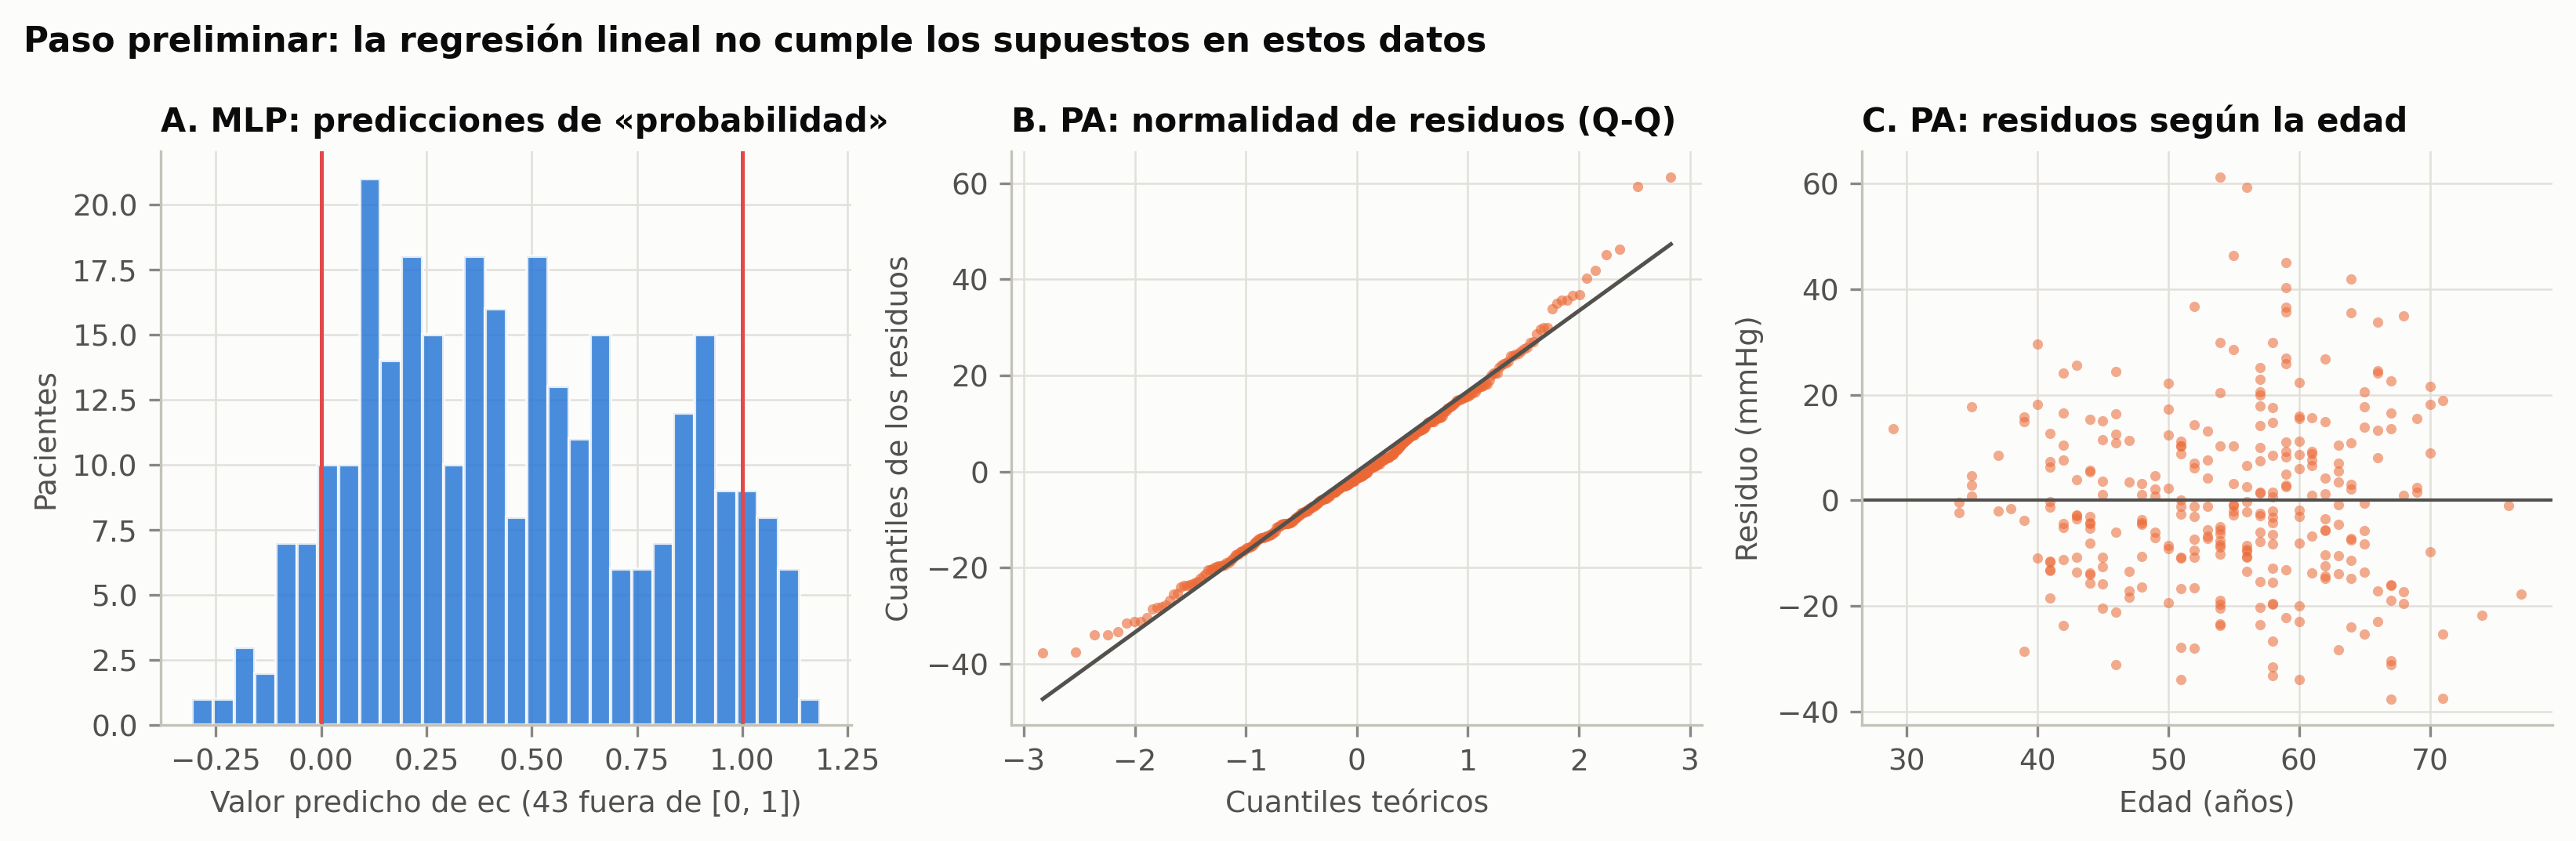
\includegraphics[width=0.92\textwidth]{fig12_regresion_lineal_preliminar.png}
\caption{Paso preliminar. (A) El MLP predice ``probabilidades'' fuera de [0,\,1]. (B) Gr\'afico Q-Q de los residuos del modelo de la PAS. (C) Residuos de la PAS seg\'un la edad: la dispersi\'on crece con la edad.}
\label{fig:lineal}
\end{figure*}

\subsection{Factores asociados (H-1)}
En el an\'alisis por rangos, los marcadores de esfuerzo fueron los de mayor riesgo crudo: depresi\'on del ST $\geq1$\,mm (OR 5,06; 3,08--8,29) y FC m\'axima $<85$\,\% de la esperada (OR 4,88; 2,83--8,39). Tambi\'en fueron significativas la edad $\geq55$ a\~nos (OR 3,39) y la PAS $\geq140$\,mmHg (OR 1,72). El colesterol $\geq240$\,mg/dL no lo fue (OR 1,51; 0,95--2,38) (Tabla~\ref{tab:rangos}).

\begin{table}[H]
\centering
\caption{OR crudos por rangos cl\'inicos (tablas $2\times2$, IC 95\,\% de Woolf).}
\label{tab:rangos}
\footnotesize
\setlength{\tabcolsep}{3pt}
\begin{tabular}{lrr}
\toprule
\textbf{Rango (expuesto)} & \textbf{OR (IC 95\,\%)} & \textbf{$p$} \\
\midrule
Edad $\geq55$ a\~nos & 3,39 (2,10--5,49) & $<0{,}001$ \\
PAS $\geq140$ mmHg & 1,72 (1,05--2,79) & 0,029 \\
Colesterol $\geq240$ mg/dL & 1,51 (0,95--2,38) & 0,080 \\
FC m\'ax.\ $<85$\,\% de la esperada & 4,88 (2,83--8,39) & $<0{,}001$ \\
Depresi\'on del ST $\geq1$ mm & 5,06 (3,08--8,29) & $<0{,}001$ \\
FC m\'ax.\ $\leq162$ lpm\ra & 4,67 (2,65--8,23) & $<0{,}001$ \\
\bottomrule
\multicolumn{3}{l}{\scriptsize \ra Corte de la fase previa; con la etiqueta invertida se hab\'ia concluido lo contrario.}
\end{tabular}
\end{table}

En el modelo multivariable b\'asico se rechaz\'o H0 de H-1 (raz\'on de verosimilitud $\chi^2=174{,}7$; gl $=14$; $p<0{,}001$; $R^2$ de Nagelkerke $=0{,}594$). Los supuestos se cumplieron: Box-Tidwell con $p\geq0{,}22$, VIF $\leq4{,}2$ y Hosmer-Lemeshow con $p=0{,}53$. Los predictores independientes fueron el dolor asintom\'atico, el sexo masculino y la depresi\'on del ST; la FC m\'axima fue protectora pero lim\'itrofe, con $p=0{,}048$ en el modelo principal y $p=0{,}051$ en el an\'alisis de sensibilidad con $n=303$ (Tabla~\ref{tab:or}, Fig.~\ref{fig:forest}). La edad, la angina de esfuerzo y la pendiente del ST perdieron significancia al ajustar. En el modelo extendido dominaron el n\'umero de vasos (OR 3,71 por vaso) y el defecto reversible en la gammagraf\'ia con talio (OR 4,03).

\begin{table*}[t]
\centering
\caption{OR crudos y ajustados (regresi\'on log\'istica por m\'axima verosimilitud). Referencias: angina t\'ipica, pendiente ascendente y talio normal.}
\label{tab:or}
\small
\begin{tabular}{lrrrrrr}
\toprule
\textbf{Variable} & \textbf{OR crudo (IC 95\,\%)} & \textbf{$p$} & \textbf{OR ajustado b\'asico} & \textbf{$p$} & \textbf{OR ajustado extendido} & \textbf{$p$} \\
\midrule
Edad (por 10 a\~nos) & 1,70 (1,29--2,23) & $<0{,}001$ & 1,25 (0,82--1,91) & 0,294 & 0,87 (0,54--1,42) & 0,580 \\
Sexo masculino & 3,57 (2,10--6,10) & $<0{,}001$ & \textbf{7,48 (3,25--17,20)} & $<0{,}001$ & 4,66 (1,66--13,08) & 0,003 \\
Dolor: angina at\'ipica & 0,51 (0,16--1,62) & 0,255 & 2,68 (0,66--10,81) & 0,166 & 3,47 (0,77--15,69) & 0,107 \\
Dolor: no anginoso & 0,63 (0,23--1,77) & 0,384 & 1,47 (0,44--4,96) & 0,533 & 1,28 (0,35--4,71) & 0,705 \\
Dolor: asintom\'atico & 6,04 (2,31--15,79) & $<0{,}001$ & \textbf{10,60 (3,17--35,40)} & $<0{,}001$ & 8,08 (2,19--29,83) & 0,002 \\
PAS (por 10 mmHg) & 1,19 (1,05--1,36) & 0,009 & 1,21 (0,99--1,47) & 0,059 & 1,28 (1,02--1,59) & 0,029 \\
Colesterol (por 40 mg/dL) & 1,13 (0,95--1,36) & 0,170 & 1,21 (0,92--1,58) & 0,175 & 1,19 (0,87--1,63) & 0,268 \\
Glucemia $>120$ mg/dL & 1,02 (0,53--1,95) & 0,956 & 0,94 (0,36--2,42) & 0,894 & 0,55 (0,17--1,81) & 0,325 \\
ECG de reposo anormal & 2,02 (1,27--3,21) & 0,003 & 1,46 (0,75--2,84) & 0,259 & 1,61 (0,76--3,41) & 0,210 \\
FC m\'axima (por 10 lpm) & 0,64 (0,56--0,73) & $<0{,}001$ & \textbf{0,82 (0,68--1,00)} & 0,048 & 0,84 (0,67--1,04) & 0,107 \\
Angina de esfuerzo & 7,00 (4,02--12,19) & $<0{,}001$ & 1,90 (0,89--4,07) & 0,098 & 2,03 (0,86--4,82) & 0,107 \\
Depresi\'on del ST (por mm) & 2,50 (1,91--3,28) & $<0{,}001$ & \textbf{1,82 (1,23--2,69)} & 0,003 & 1,43 (0,92--2,25) & 0,115 \\
Pendiente del ST plana & 5,30 (3,16--8,90) & $<0{,}001$ & 2,11 (0,95--4,72) & 0,068 & 3,17 (1,25--8,02) & 0,015 \\
Pendiente del ST descendente & 3,81 (1,48--9,80) & 0,005 & 0,69 (0,12--3,80) & 0,668 & 1,68 (0,28--10,19) & 0,572 \\
Vasos por fluoroscopia (por vaso) & 3,48 (2,46--4,93) & $<0{,}001$ & --- & --- & 3,71 (2,15--6,41) & $<0{,}001$ \\
Talio: defecto fijo & 6,86 (2,41--19,54) & $<0{,}001$ & --- & --- & 0,99 (0,21--4,64) & 0,987 \\
Talio: defecto reversible & 11,19 (6,35--19,70) & $<0{,}001$ & --- & --- & 4,03 (1,75--9,27) & 0,001 \\
\bottomrule
\end{tabular}
\end{table*}

\begin{figure*}[t]
\centering
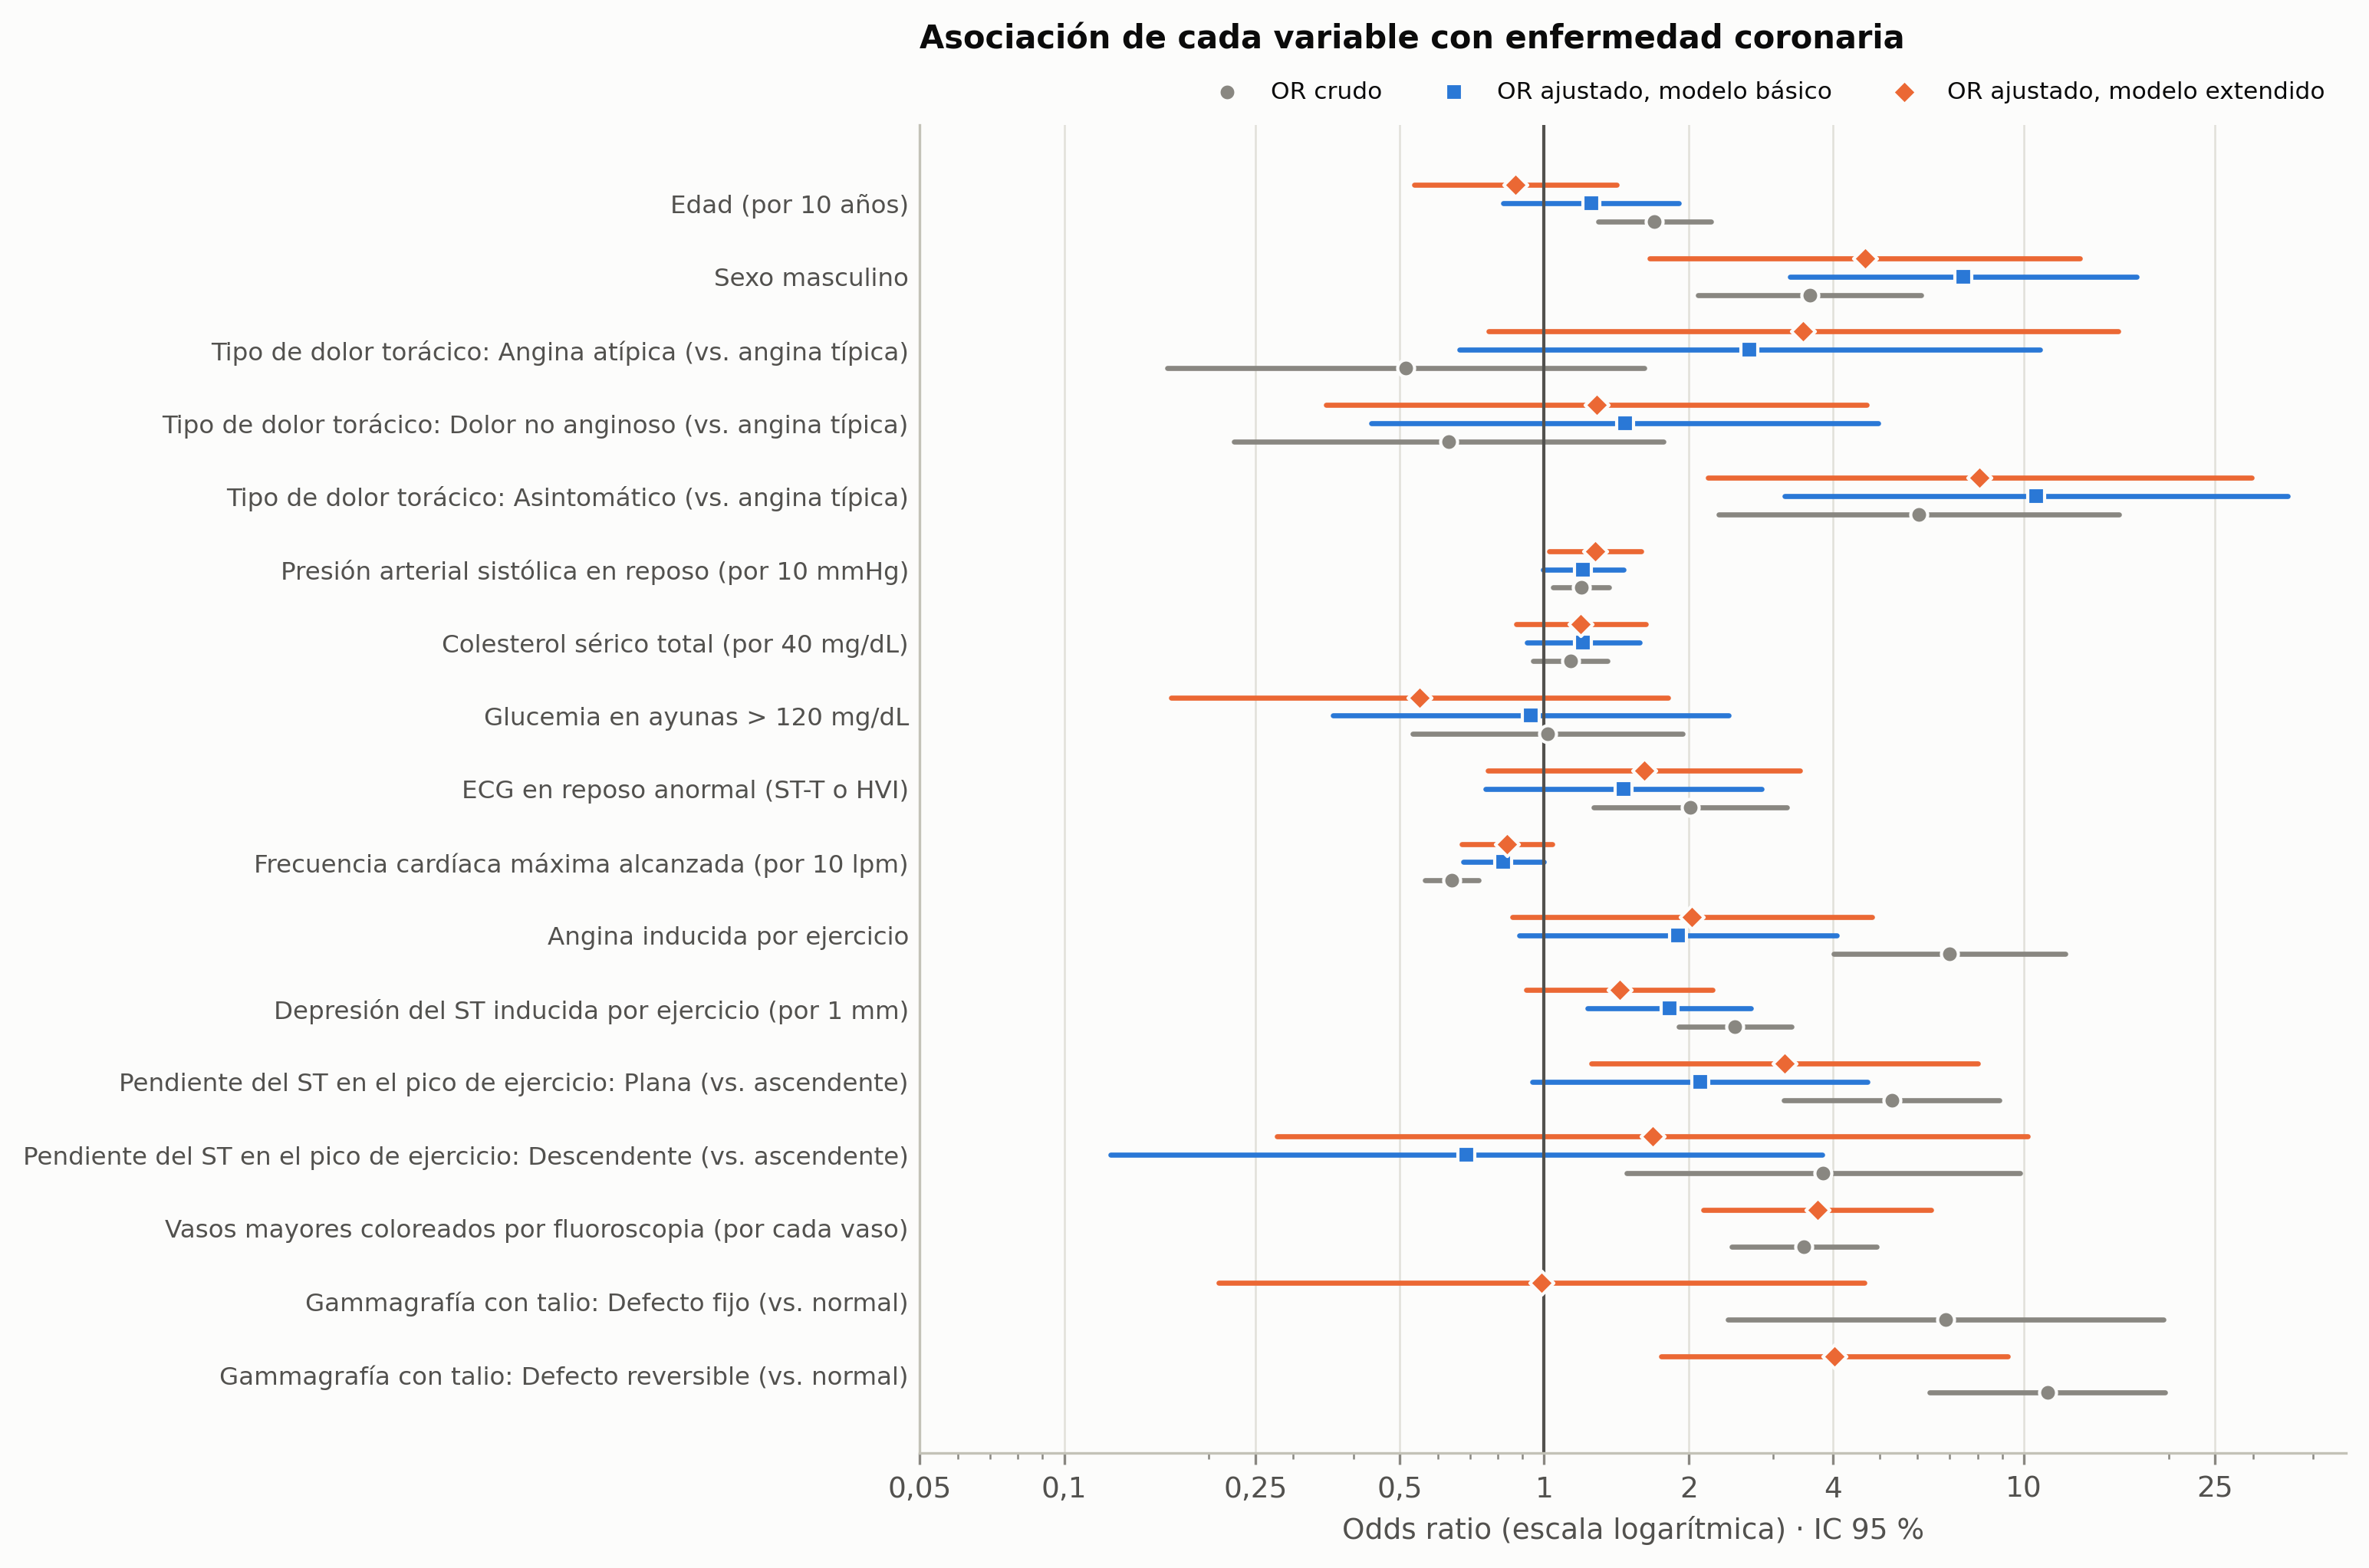
\includegraphics[width=0.78\textwidth]{fig06_forest_odds_ratios.png}
\caption{OR crudos (gris) y ajustados en los modelos b\'asico (azul) y extendido (naranja), en escala logar\'itmica.}
\label{fig:forest}
\end{figure*}

\subsection{Desempe\~no predictivo (H-2 a H-4)}
El modelo b\'asico alcanz\'o un AUC de 0,874 en validaci\'on cruzada, con IC de DeLong de 0,836 a 0,914 y un AUC de 0,880 corregido por optimismo (optimismo de 0,021). Por tanto, se rechaza H0 de H-2. Su pendiente de calibraci\'on fue de 0,91 (Tabla~\ref{tab:desempeno}, Figs.~\ref{fig:roc} y~\ref{fig:calib}). La imagen aument\'o el AUC en 0,035 (IC 95\,\% 0,008--0,062; $p=0{,}012$), y se rechaza H0 de H-3. La RL extendida super\'o al \'arbol ($\Delta$AUC 0,067; IC 0,021--0,113; $p=0{,}004$), y se rechaza H0 de H-4. No difiri\'o del Random Forest ($\Delta$AUC $-0{,}001$; $p=0{,}94$). El \'arbol estuvo sobreajustado (pendiente de calibraci\'on de 0,26) y fue inestable: sus hiperpar\'ametros modales (profundidad 4, hojas de al menos 10 pacientes) se eligieron solo en el 32\,\% de las particiones. Con 4 variables (M0), el AUC fue de 0,749, de modo que M1 lo mejor\'o en 0,125 ($p<0{,}001$).

\begin{table*}[t]
\centering
\caption{Desempe\~no en validaci\'on cruzada $5\times20$ (media y percentiles 2,5--97,5) y con predicciones fuera de muestra.}
\label{tab:desempeno}
\small
\begin{tabular}{lcccccc}
\toprule
\textbf{Modelo} & \textbf{AUC CV} & \textbf{AUC (IC DeLong)} & \textbf{Brier} & \textbf{Pend.\ calib.} & \textbf{Sens./Esp.\ (0,5)} & \textbf{Esp.\ (sens.\ $\geq$90\,\%)} \\
\midrule
M0 RL 4 continuas & 0,749 (0,612--0,865) & 0,746 (0,690--0,801) & 0,205 & 0,93 & 0,650 / 0,769 & 0,344 \\
\textbf{M1 RL b\'asica} & \textbf{0,874 (0,794--0,949)} & \textbf{0,875 (0,836--0,914)} & 0,146 & \textbf{0,91} & 0,752 / 0,844 & 0,613 \\
M2 RL extendida & 0,909 (0,829--0,964) & 0,904 (0,870--0,938) & 0,120 & 0,84 & 0,788 / 0,875 & 0,700 \\
M3 \'Arbol CART & 0,842 (0,715--0,940) & 0,847 (0,802--0,893) & 0,163 & 0,26 & 0,737 / 0,875 & 0,519 \\
M4 Random Forest & 0,910 (0,833--0,964) & 0,905 (0,872--0,938) & 0,127 & 1,59 & 0,759 / 0,875 & 0,719 \\
\bottomrule
\end{tabular}
\end{table*}

\begin{figure}[H]
\centering
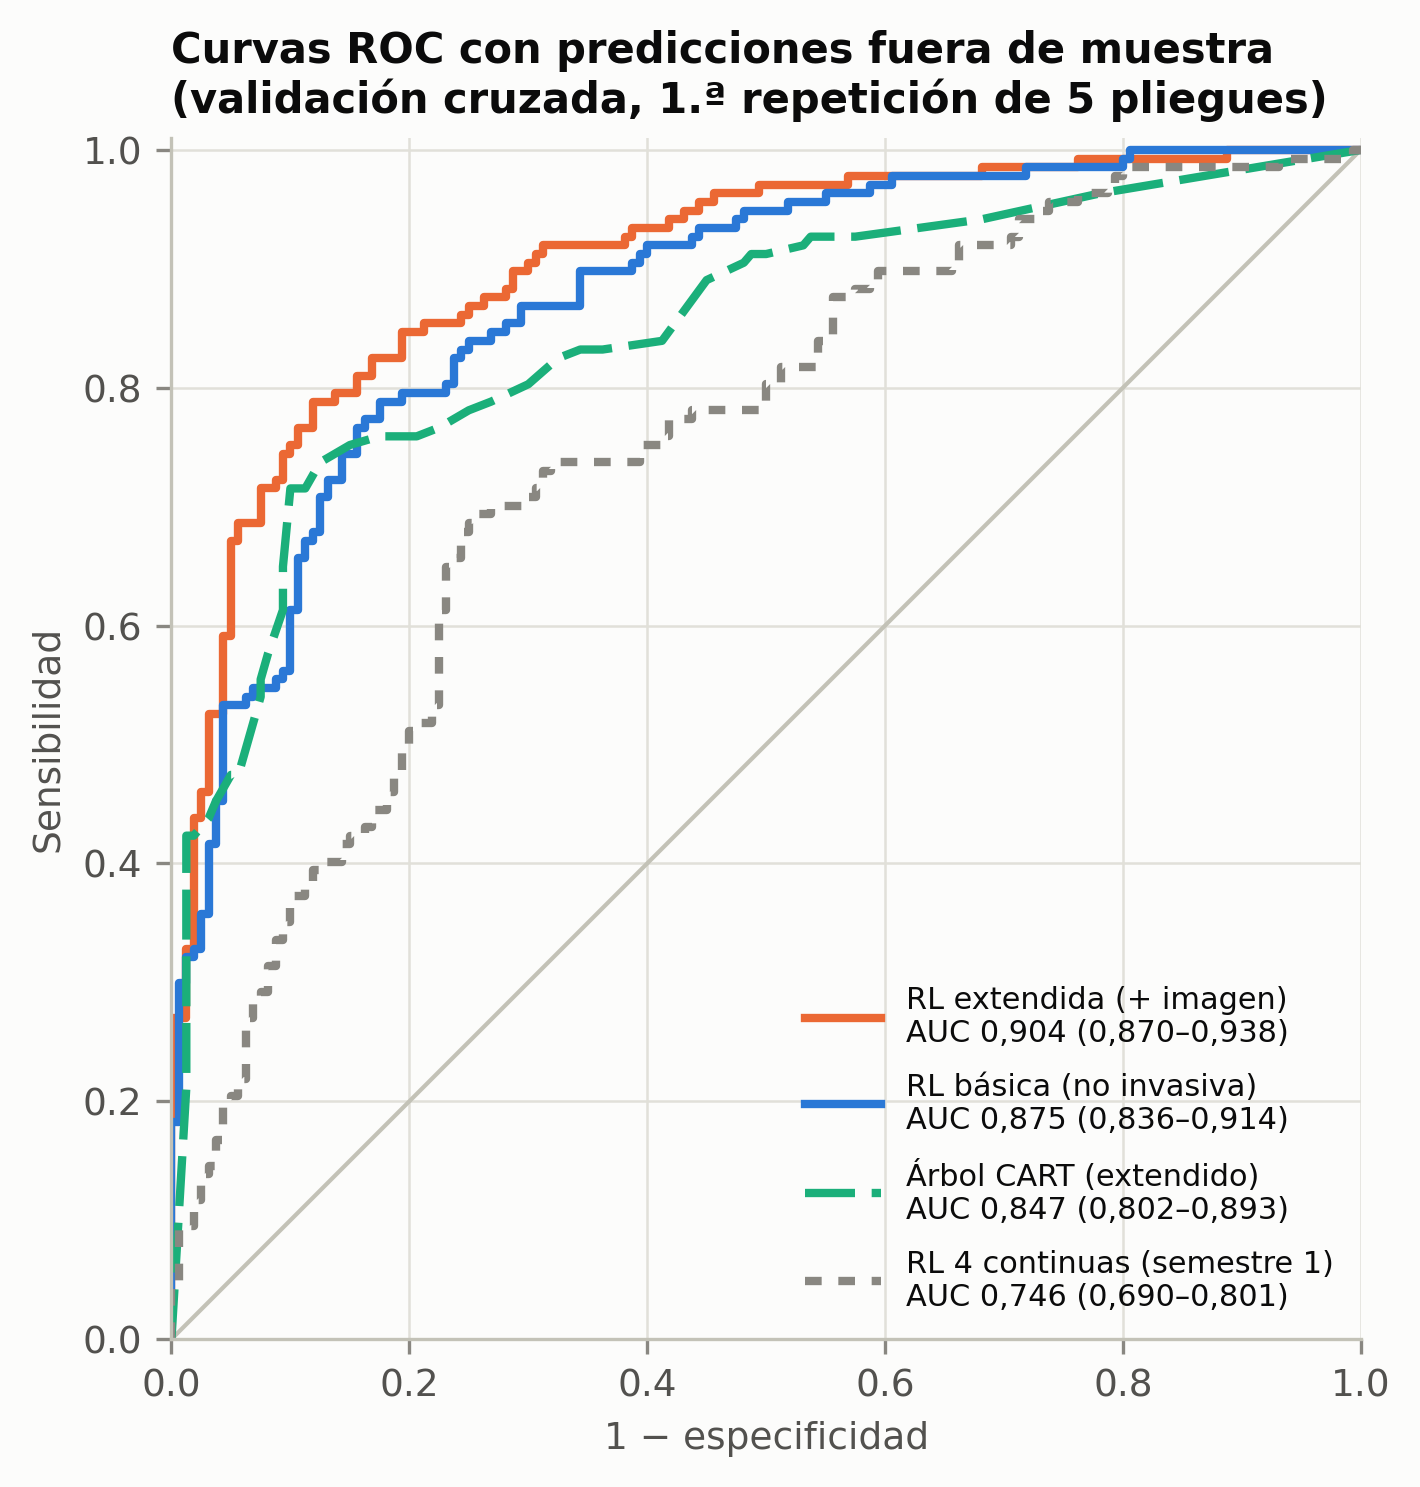
\includegraphics[width=0.9\columnwidth]{fig07_curvas_roc.png}
\caption{Curvas ROC con predicciones fuera de muestra.}
\label{fig:roc}
\end{figure}

\begin{figure}[H]
\centering
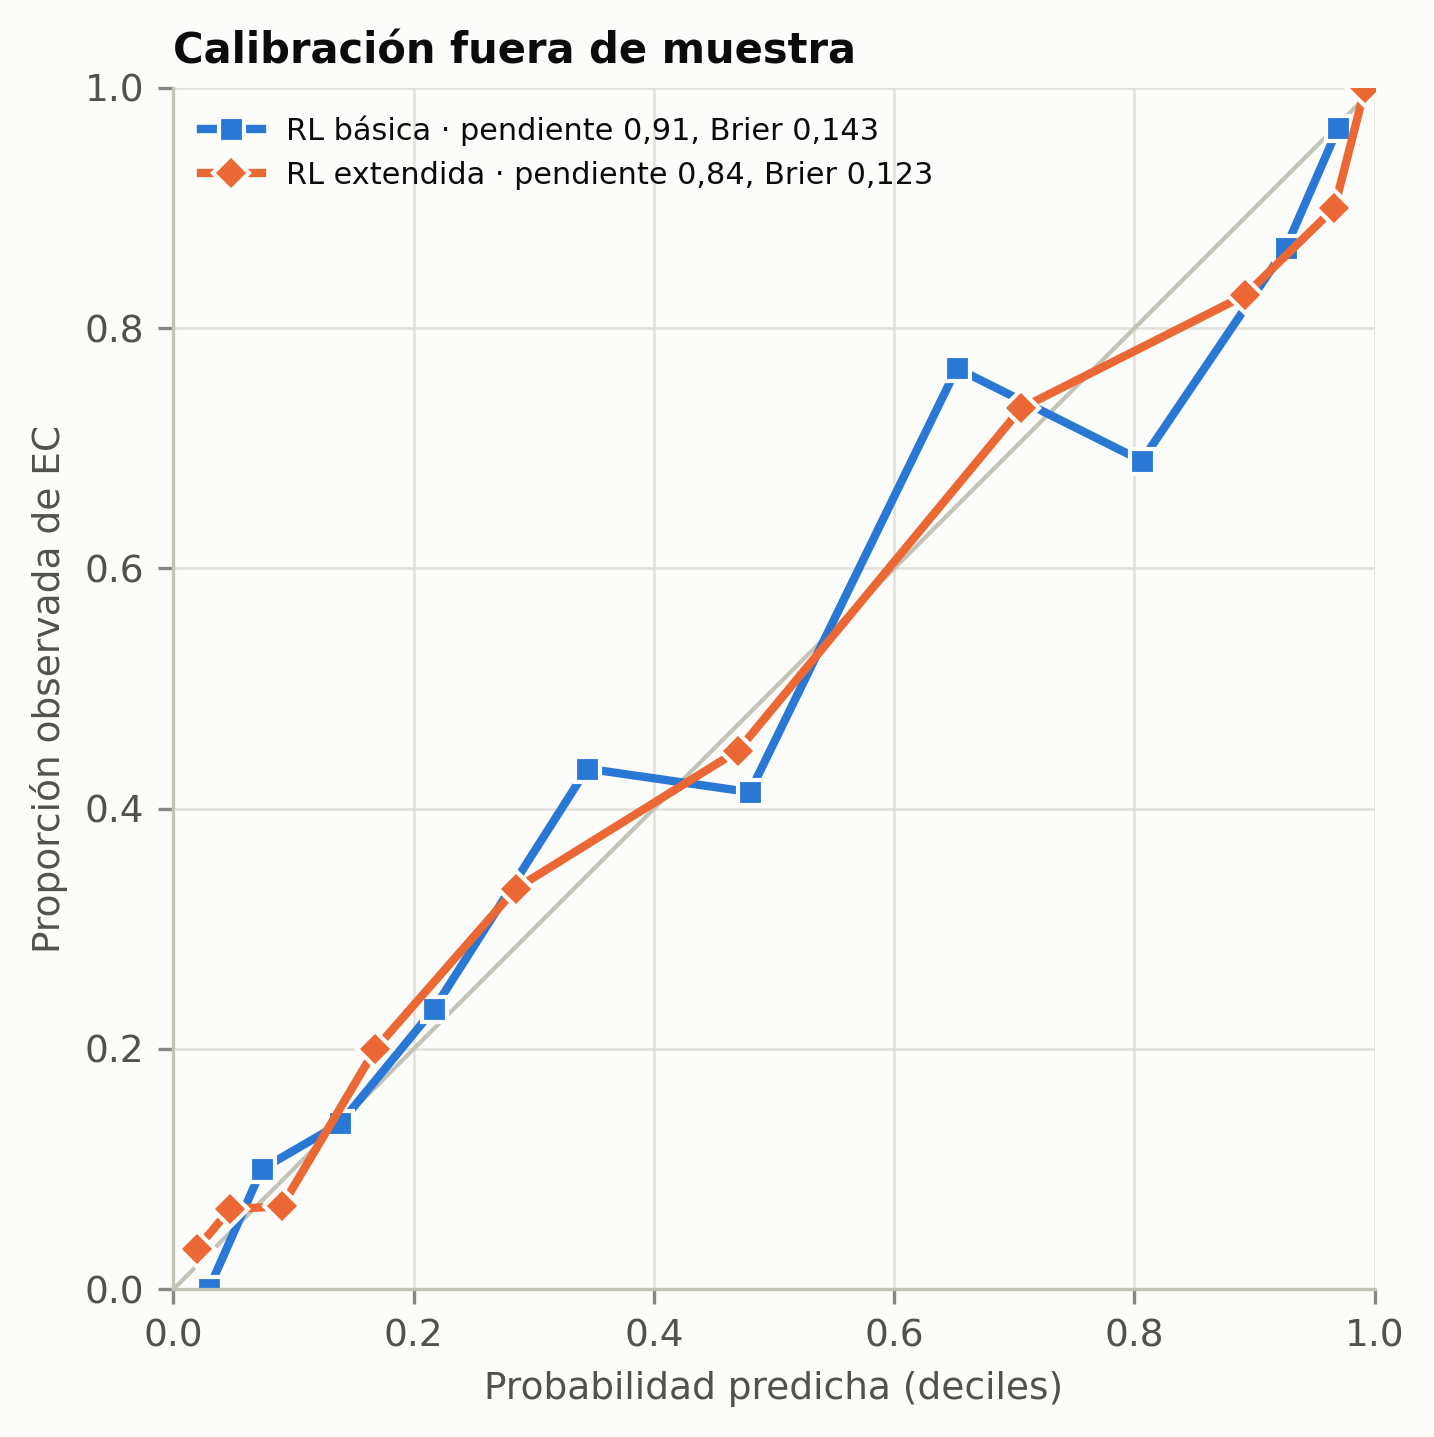
\includegraphics[width=0.85\columnwidth]{fig08_calibracion.png}
\caption{Calibraci\'on fuera de muestra (deciles de riesgo).}
\label{fig:calib}
\end{figure}

\begin{figure}[H]
\centering
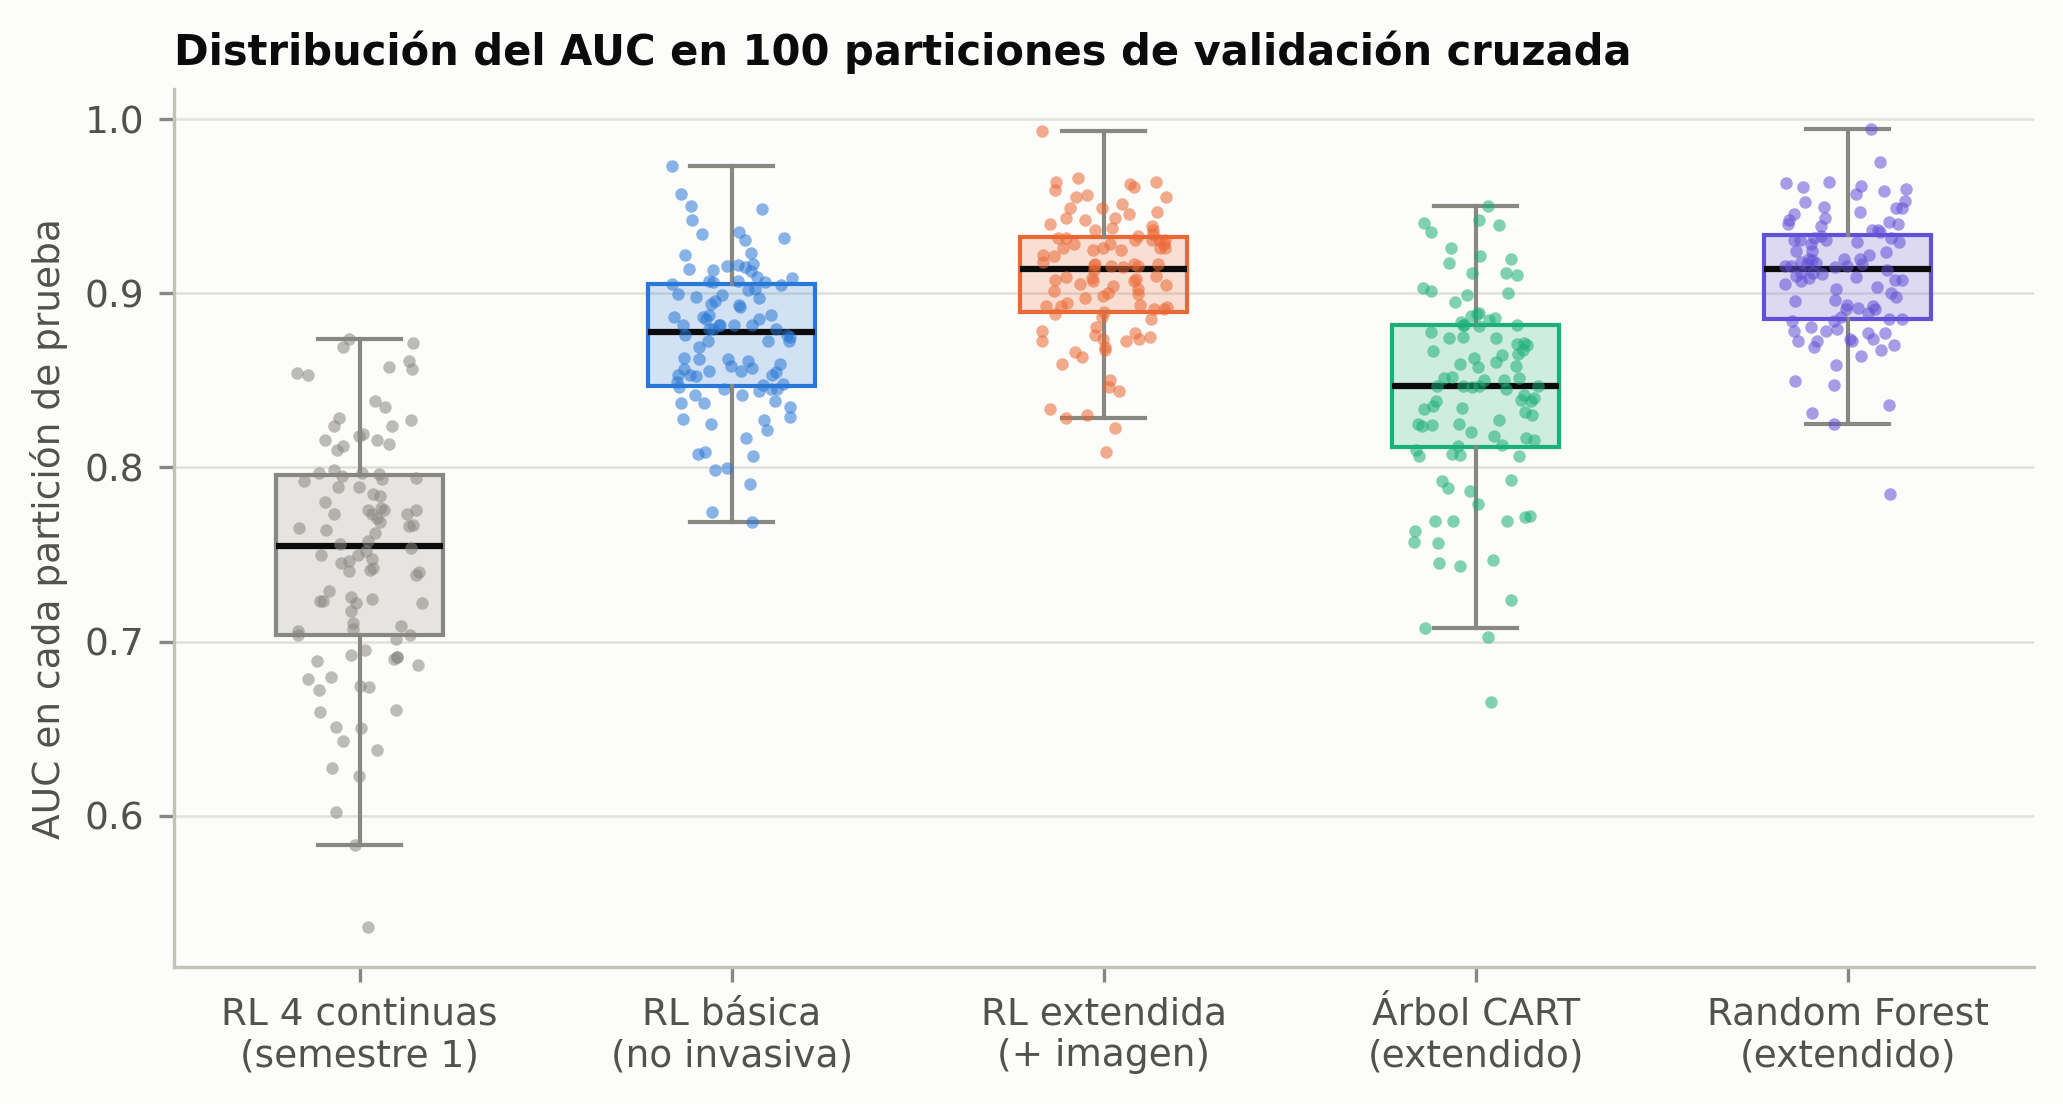
\includegraphics[width=\columnwidth]{fig10_auc_validacion_cruzada.png}
\caption{AUC en cada una de las 100 particiones: una sola partici\'on puede dar resultados muy distintos.}
\label{fig:cv}
\end{figure}

Con el umbral que garantiza una sensibilidad del 90\,\% (0,24), el modelo b\'asico detect\'o 124 de 137 enfermos y descart\'o correctamente a 98 de 160 sanos (especificidad del 61,3\,\%; VPN del 88,3\,\%).

\begin{figure*}[t]
\centering
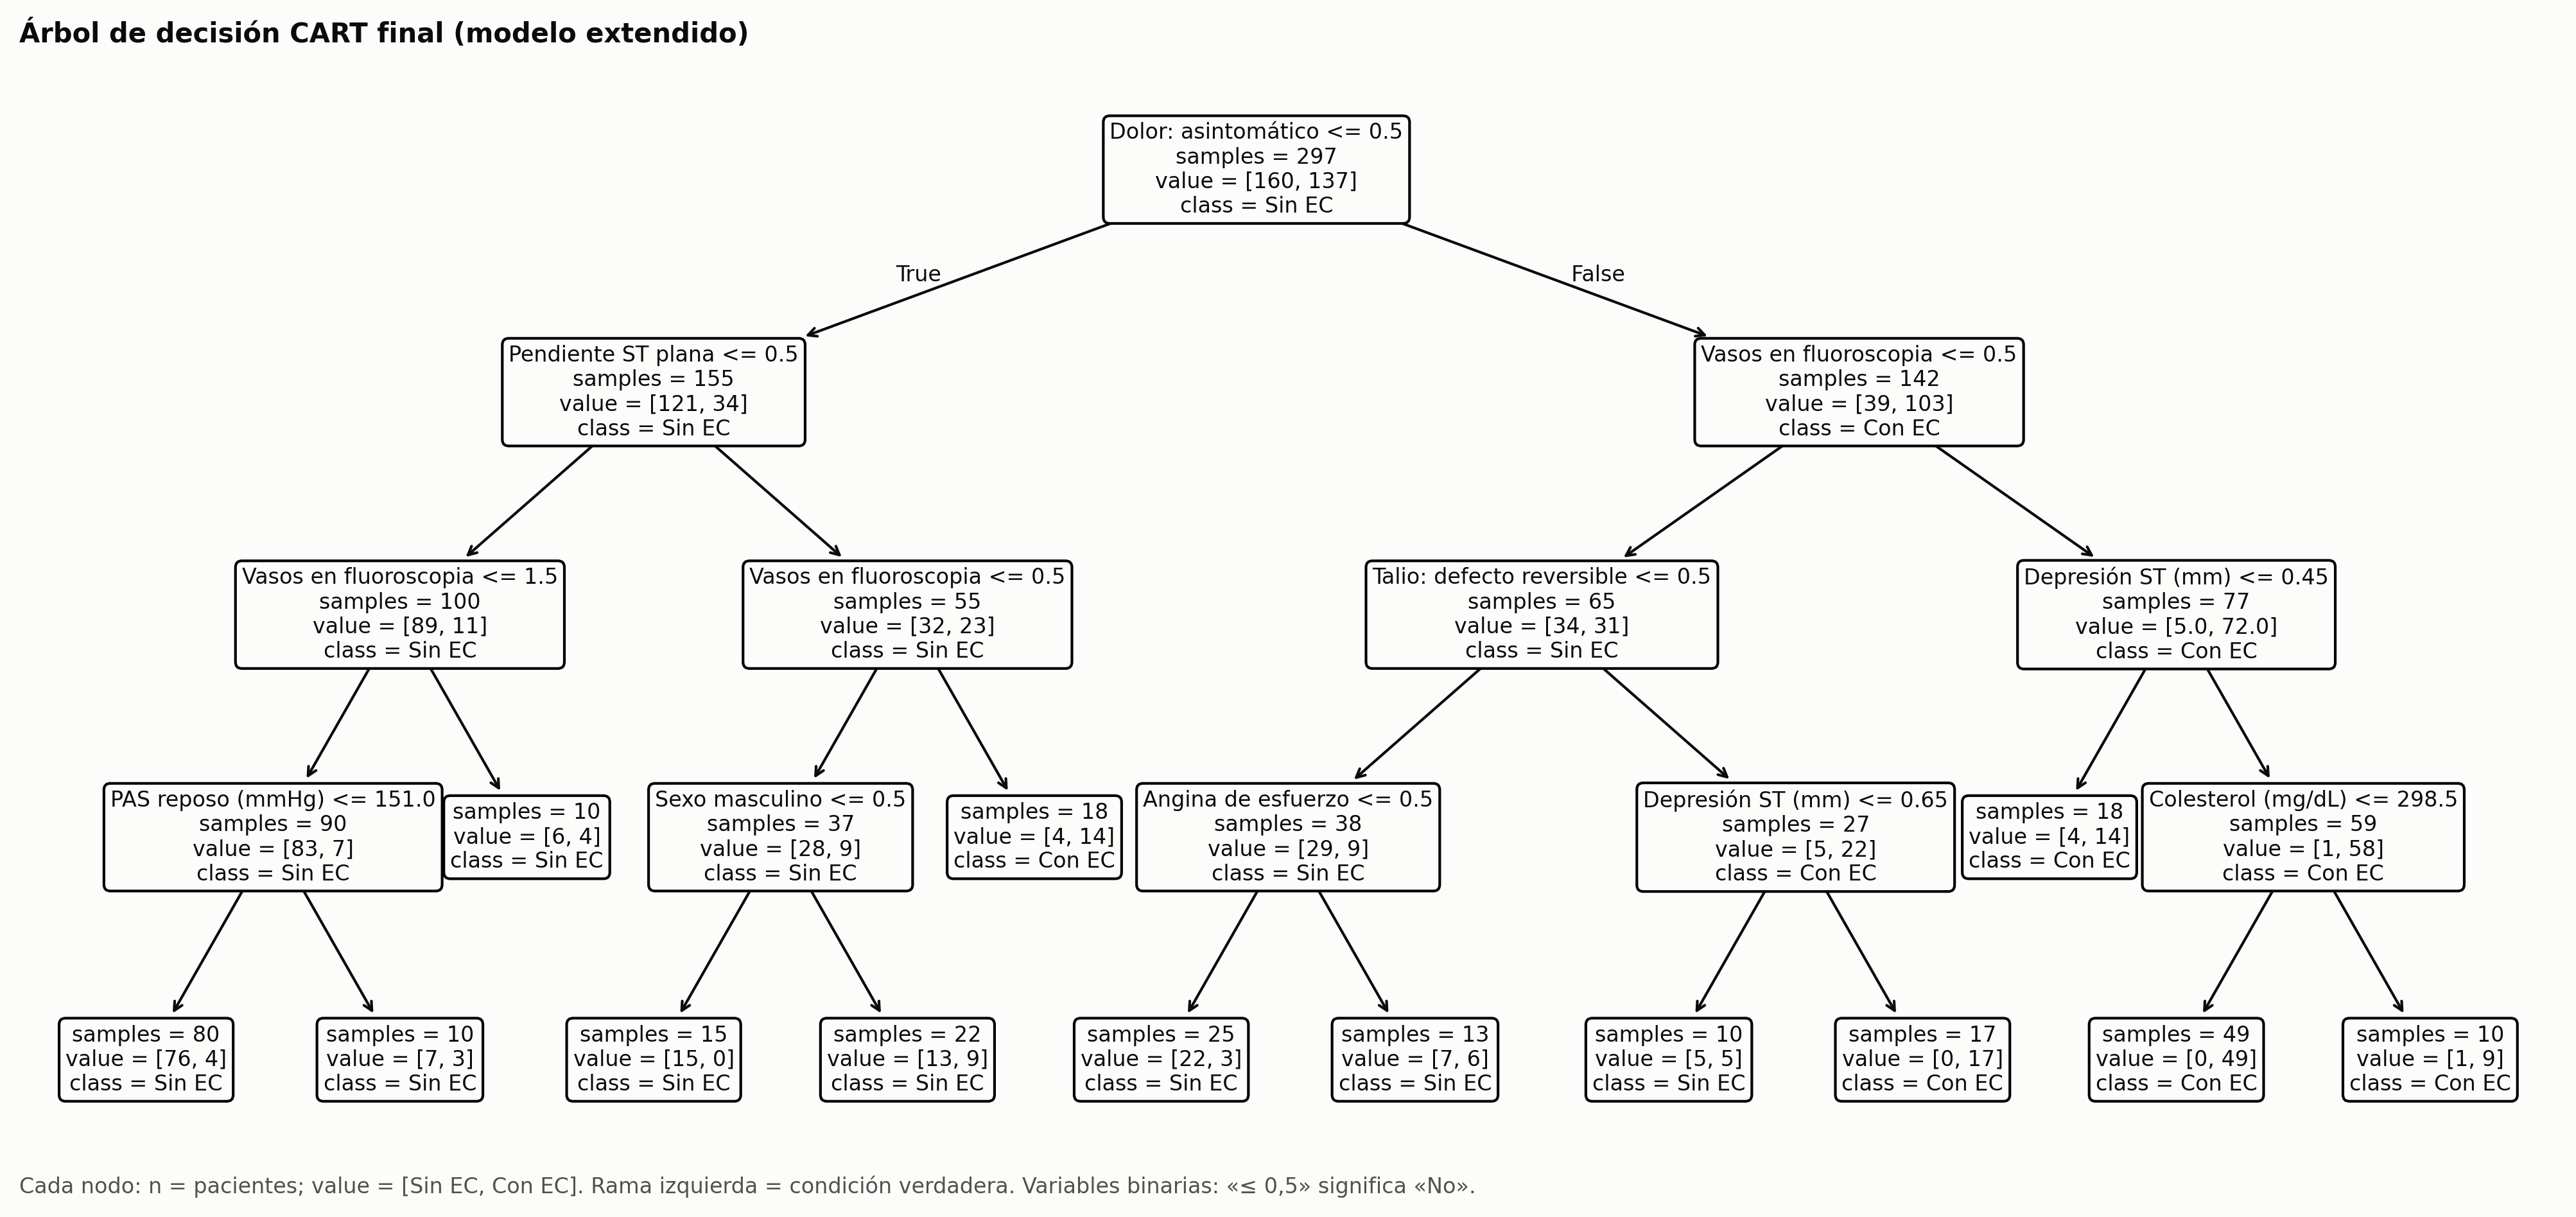
\includegraphics[width=0.95\textwidth]{fig09_arbol_decision.png}
\caption{\'Arbol CART final. La primera divisi\'on es el dolor tor\'acico asintom\'atico; le siguen el n\'umero de vasos, el talio con defecto reversible y la pendiente del ST.}
\label{fig:arbol}
\end{figure*}

%======================================================================
\section{Discusi\'on}
%======================================================================
Con informaci\'on obtenible sin imagen, un modelo log\'istico discrimina la EC con un AUC de 0,87--0,88 y buena calibraci\'on. La imagen aporta poco, y el modelo simple iguala al complejo.

\textbf{Coherencia con la literatura.} El dolor tor\'acico y el sexo son los pilares de las reglas de probabilidad pretest \cite{diamond1979,genders2011}. La asociaci\'on inversa de la FC m\'axima es fisiol\'ogica: el miocardio isqu\'emico limita la respuesta cronotr\'opica (incompetencia cronotr\'opica, OR 4,88). La depresi\'on del ST es el marcador cl\'asico de isquemia de esfuerzo \cite{vrints2024}.

\textbf{El colesterol.} Su falta de asociaci\'on se explica por tres razones: (i) el colesterol act\'ua durante d\'ecadas, mientras los marcadores de esfuerzo reflejan la enfermedad ya instaurada; (ii) en una cohorte remitida ambos grupos tienen perfiles de riesgo elevados (sesgo de espectro); y (iii) se desconoce el uso de estatinas. Esto no resta importancia al colesterol en la prevenci\'on.

\textbf{Comparaci\'on con Chandrasekhar y Peddakrishna} \cite{chandrasekhar2023}. Ellos reportaron una exactitud del 90,2\,\% y una sensibilidad del 100\,\% para la RL con 61 pacientes de prueba. Nuestras m\'etricas son menores pero m\'as robustas: la Fig.~\ref{fig:cv} muestra que el AUC del mismo modelo var\'ia entre 0,83 y 0,96 seg\'un la partici\'on, y nosotros reportamos IC, calibraci\'on y correcci\'on de optimismo. Ambos estudios coinciden en que la RL es competitiva frente a algoritmos m\'as complejos.

\textbf{Calidad de los datos.} La etiqueta invertida de la versi\'on de Kaggle hab\'ia llevado, en la fase previa del proyecto, a concluir que una FC alta era un factor de riesgo. Verificar la fuente cambi\'o las conclusiones, lo que confirma que el control de calidad es parte del m\'etodo.

\textbf{Limitaciones.}
\begin{itemize}
\item Datos de EE.\,UU. de los a\~nos 80, de pacientes remitidos (sesgo de espectro).
\item Tama\~no de muestra menor que el recomendado y predominio masculino (67,7\,\%).
\item Ausencia de tabaquismo, diabetes diagnosticada, IMC y estatinas.
\item Dise\~no transversal y validaci\'on solo interna.
\end{itemize}
Se mitigaron con penalizaci\'on, validaci\'on repetida, correcci\'on de optimismo, an\'alisis de sensibilidad y reporte de la calibraci\'on. El modelo no debe usarse cl\'inicamente sin validaci\'on externa.

\textbf{Trabajo futuro.} Validaci\'on externa con las sedes de Hungr\'ia, Suiza y Long Beach, y con datos colombianos (con aval \'etico); incorporaci\'on de factores ausentes; y an\'alisis de curva de decisi\'on.

%======================================================================
\section{Conclusiones}
%======================================================================
\begin{enumerate}
\item El sexo masculino, el dolor tor\'acico asintom\'atico y la depresi\'on del ST se asocian de forma independiente con la EC angiogr\'afica. La FC m\'axima alta es protectora, con evidencia lim\'itrofe, y el colesterol no se asoci\'o.
\item Un modelo log\'istico con 11 variables no invasivas discrimina bien (AUC de 0,874; 0,880 corregido) y est\'a bien calibrado.
\item La fluoroscopia y la gammagraf\'ia con talio mejoran la discriminaci\'on de forma significativa pero modesta (+0,035).
\item La RL supera al \'arbol de decisi\'on e iguala al Random Forest, con mejor calibraci\'on e interpretabilidad.
\item La versi\'on de Kaggle de esta base tiene la etiqueta invertida: verificar la fuente de los datos es indispensable.
\end{enumerate}

%======================================================================
\section{Administraci\'on del proyecto}
%======================================================================
\textbf{Equipo.} Angie Tobar y Alejandro Pardo (coinvestigadores), con la asesor\'ia metodol\'ogica de la Prof.\ Eliana Andrea Gonz\'alez Artunduaga.

\textbf{Instituciones.} Universidad Externado de Colombia (ejecutora), UCI Machine Learning Repository (proveedor de los datos) y Cleveland Clinic Foundation (origen de los datos).

\textbf{Cronograma.}
\begin{itemize}
\item \textbf{Semestre 1 (feb--may 2026):} selecci\'on de la base, exploraci\'on, primeros modelos y presentaci\'on.
\item \textbf{Semestre 2 (ago--nov 2026):} ficha de la base; estructura del proyecto; auditor\'ia y migraci\'on a la base oficial; rean\'alisis; documento final; exposici\'on (3--14 nov).
\end{itemize}

\textbf{Presupuesto} (referencial). El costo total estimado es de \$8.977.500 COP:
\begin{itemize}
\item personal: 2 investigadores $\times$ 120 h, \$6.000.000;
\item asesor\'ia: 20 h, \$1.800.000;
\item equipos: \$400.000;
\item datos y software libres: \$0;
\item divulgaci\'on: \$150.000;
\item administrativos: \$200.000;
\item imprevistos (5\,\%): \$427.500.
\end{itemize}
El 94\,\% es aporte en especie y contrapartida institucional, sin financiaci\'on externa.

%======================================================================
\begin{thebibliography}{99}
\small
\bibitem{ihme2025} Institute for Health Metrics and Evaluation. Cardiovascular diseases caused 1 in 3 global deaths in 2023. Seattle: IHME; 2025.
\bibitem{stark2024} Stark B, Johnson C, Roth GA. Global prevalence of coronary artery disease: an update from the Global Burden of Disease Study. J Am Coll Cardiol. 2024;83(13 Suppl):2320.
\bibitem{deloitte2015} Deloitte; Revista Semana. El costo de las enfermedades del coraz\'on en Colombia. Bogot\'a; 2015.
\bibitem{rcc2018} Revista Colombiana de Cardiolog\'ia. Estimaci\'on de los costos directos de los eventos coronarios en Colombia. Rev Colomb Cardiol. 2018.
\bibitem{vrints2024} Vrints C, Andreotti F, Koskinas KC, Rossello X, Adamo M, Ainslie J, et al. 2024 ESC Guidelines for the management of chronic coronary syndromes. Eur Heart J. 2024;45(36):3415-537.
\bibitem{diamond1979} Diamond GA, Forrester JS. Analysis of probability as an aid in the clinical diagnosis of coronary-artery disease. N Engl J Med. 1979;300(24):1350-8.
\bibitem{detrano1989} Detrano R, Janosi A, Steinbrunn W, Pfisterer M, Schmid JJ, Sandhu S, et al. International application of a new probability algorithm for the diagnosis of coronary artery disease. Am J Cardiol. 1989;64(5):304-10.
\bibitem{genders2011} Genders TSS, Steyerberg EW, Alkadhi H, Leschka S, Desbiolles L, Nieman K, et al. A clinical prediction rule for the diagnosis of coronary artery disease: validation, updating, and extension. Eur Heart J. 2011;32(11):1316-30.
\bibitem{chandrasekhar2023} Chandrasekhar N, Peddakrishna S. Enhancing heart disease prediction accuracy through machine learning techniques and optimization. Processes. 2023;11(4):1210.
\bibitem{vancalster2019} Van Calster B, McLernon DJ, van Smeden M, Wynants L, Steyerberg EW. Calibration: the Achilles heel of predictive analytics. BMC Med. 2019;17(1):230.
\bibitem{collins2015} Collins GS, Reitsma JB, Altman DG, Moons KGM. Transparent reporting of a multivariable prediction model for individual prognosis or diagnosis (TRIPOD): the TRIPOD statement. BMJ. 2015;350:g7594.
\bibitem{uci1988} Janosi A, Steinbrunn W, Pfisterer M, Detrano R. Heart Disease [dataset]. UCI Machine Learning Repository; 1988. doi:10.24432/C52P4X.
\bibitem{riley2020} Riley RD, Ensor J, Snell KIE, Harrell FE Jr, Martin GP, Reitsma JB, et al. Calculating the sample size required for developing a clinical prediction model. BMJ. 2020;368:m441.
\bibitem{shapiro1965} Shapiro SS, Wilk MB. An analysis of variance test for normality (complete samples). Biometrika. 1965;52(3-4):591-611.
\bibitem{hosmer2013} Hosmer DW, Lemeshow S, Sturdivant RX. Applied logistic regression. 3rd ed. Hoboken (NJ): Wiley; 2013.
\bibitem{pedregosa2011} Pedregosa F, Varoquaux G, Gramfort A, Michel V, Thirion B, Grisel O, et al. Scikit-learn: machine learning in Python. J Mach Learn Res. 2011;12:2825-30.
\bibitem{breiman1984} Breiman L, Friedman JH, Olshen RA, Stone CJ. Classification and regression trees. Belmont (CA): Wadsworth; 1984.
\bibitem{breiman2001} Breiman L. Random forests. Mach Learn. 2001;45(1):5-32.
\bibitem{harrell2015} Harrell FE Jr. Regression modeling strategies. 2nd ed. Cham: Springer; 2015.
\bibitem{delong1988} DeLong ER, DeLong DM, Clarke-Pearson DL. Comparing the areas under two or more correlated receiver operating characteristic curves: a nonparametric approach. Biometrics. 1988;44(3):837-45.
\bibitem{sun2014} Sun X, Xu W. Fast implementation of DeLong's algorithm for comparing the areas under correlated receiver operating characteristic curves. IEEE Signal Process Lett. 2014;21(11):1389-93.
\bibitem{nadeau2003} Nadeau C, Bengio Y. Inference for the generalization error. Mach Learn. 2003;52(3):239-81.
\bibitem{seabold2010} Seabold S, Perktold J. Statsmodels: econometric and statistical modeling with Python. In: Proceedings of the 9th Python in Science Conference; 2010. p. 92-6.
\bibitem{res8430} Ministerio de Salud de Colombia. Resoluci\'on 8430 de 1993. Bogot\'a; 1993.
\bibitem{ley1581} Congreso de la Rep\'ublica de Colombia. Ley Estatutaria 1581 de 2012. Bogot\'a; 2012.
\end{thebibliography}

\end{document}
